% Rozdziały zaczynają się od "chapter"
\chapter{Wprowadzenie}
% Praca podzielona na mniejsze pliki włączane za pomocą input
% Zajrzyj do pliku tekst/wstep.tex
Głównym celem każdej aplikacji cyfrowej, systemu informatycznego czy innego rodzaju usług dostępnych przez sieć jest przetwarzanie informacji cyfrowej. Dzięki dygitalizacji usług oraz utworzeniu kompletnie nowych jej rodzajów zależnych od technologii cyfrowych ludzkość generuje masywne ilości danych każdego dnia. Jednym~z~najpopularniejszych środków komunikacji, zwłaszcza dla biznesu, jest poczta elektroniczna. Grupa \textbf{Radicati Inc.} spekuluje, że do końca 2023 liczba wysłanych listów elektronicznych powinna przekroczyć 347 miliardów \cite{radicati2019}.
\textbf{Domo, Inc}, które jest jednym~z~wielu dostawców usług chmurowych,~w~swoim raporcie zatytułowanym 
\foreignquote{english}{Data Never Sleeps 10.0} donosi o tym, że wielkość danych, które zostaną utworzone czy skopiowane może wejść~w~okolicę 181 zettabajtów\footnote{Zetta bajt (skrót \textbf{ZB})~w~systemie SI to tryliard $10^{21}$ bajtów~i~$2^{70}$, czyli $1024^{7}$ bajtów.} wielkości do roku 2025 \cite{domo10}. Znakomita część tych danych musi być przechowywana na stałe, gdyż wymaga tego poprawne działanie systemu lub może wynikać~z~nakazów prawnych.~Z~tych powodów jednym~z~priorytetów przy administracji systemu jest zabezpieczenie przed utratą danych przez instytucje~i~działalności gospodarcze.
Do powodów utraty danych mogą należeć:
\begin{itemize}
    \item awaria nośników~i~innych elementów,
    \item niespodziewane braki~w~dostawach prądu,
    \item błąd ludzki,
    \item wirusy komputerowe.
\end{itemize}

%%%%%%%%%%%%%%%%%%%%%%%%%%%%%%%%%%%%%%%%%%%%%%%%
\section{Cel pracy}
Celem tej pracy było odnalezienie sposobu na zniwelowanie strat danych~w~wyniku ataku wirusa typu ransomware możliwego do wykorzystania przez administratorów~w~warunkach rzeczywistego ataku. Zaproponowanym przeze mnie rozwiązaniem jest \foreignquote{english}{proof of concept} w postaci oprogramowania analizującego działania na plikach dla systemów operacyjnych~z~rodziny Linux.
%Celem tej pracy było utworzenie oprogramowania, które zajmuje się niwelowaniem ryzyka utraty danych~z~powodu ataku wirusa komputerowego typu ransomware na systemach~z~rodziny Linux oraz przetestowanie jego działania~w~trakcie rzeczywistego ataku.
 Program korzysta~z~informacji o stanie systemu plików~i~na bieżąco analizuje wykonywane na nim operacje. Statystyki~z~obserwowanego obszaru zawierają~w~sobie m.in. ilości operacji, ścieżkę do użytej komendy, nazwę użytkownika, który dokonuje operacji etc. Dzięki temu administrator może nie tylko dowiedzieć się o potencjalnym zagrożeniu ataku ransomware, ale też obserwować dowolny, podejrzany ruch na systemie plików. Następnie dokonywana jest analiza zawartości plików~i~generowany jest raport o zakresie ryzyka.
Docelową grupą użytkowników są administratorzy,~a~więc główne założenia, jakie postawiłem sobie~w~trakcie tworzenia rozwiązania, miały na celu wytworzenie oprogramowania łatwego dla nich~w~obsłudze. Tymi założeniami są:
\begin{itemize}
    \item łatwa instalacja, która nie wymaga aktualizacji sterowników sprzętowych,
    \item wsparcie dla najpopularniejszych dystrybucji serwerowych\footnote{W3 Techs utrzymuje raport o sieciowych serwerach Linuksowych. Jest on codziennie aktualizowany~i~można go odnaleźć pod adresem: \url{https://w3techs.com/technologies/details/os-linux}},
    \item minimalne zużycie zasobów,
    \item integracja~z~bieżącymi popularnymi rozwiązaniami~w~administracji systemów.
\end{itemize}

%%%%%%%%%%%%%%%%%%%%%%%%%%%%%%%%%%%%%%%%%%%%%%%%
\section{Opis problemu~i~znaczenie zagrożeń typu ransomware}
 Od 2017 roku obserwuje się trend wzrostowy ataków ransomware\cite{petrosyan_worldwide_nodate}, a~w~ciągu pierwszej połowy 2022 roku, dokonano 236,7 miliona ataków na całym świecie 
 \cite{petrosyan_number_nodate}. Wg. raportu Verizona \footnote{Raport jest odpłatnie dostępny pod linkiem: \url{https://www.verizon.com/business/resources/reports/dbir/2021/results-and-analysis}} ataki ransomware stanowią 10\% wszystkich naruszeń danych~w~2021. Wedle zebranych statystyk wykrycie ich zajęło~w~aż 49 dni dłużej niż średni czas wykrycia wszystkich naruszeń~z~tego samego roku. Raport wyjaśnia też, że zagrożona nie jest wyłącznie branża IT, ale też inne sektory,~w~szczególności sektor ochrony zdrowia.
\begin{figure}[H]
     \centering
     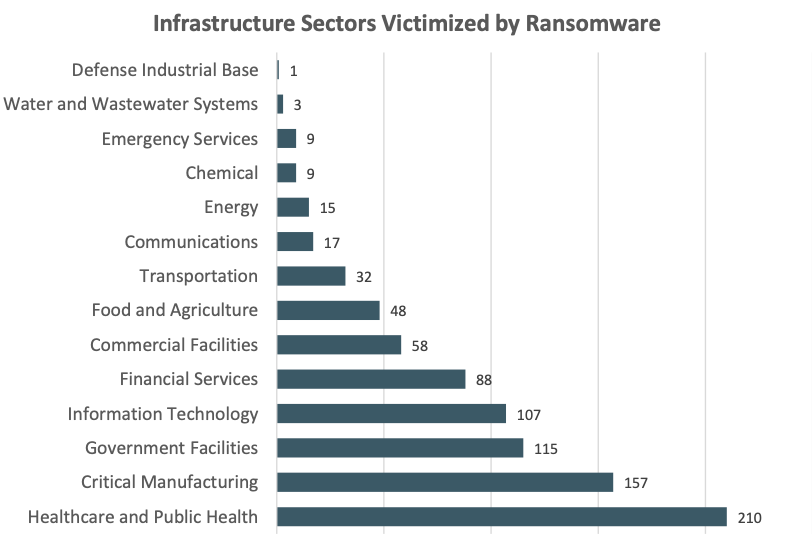
\includegraphics[width=0.78\linewidth]{rysunki/attacks_on_sectors.png}
     \caption{Sektory infrastruktury krytycznej, do których odnosiły się skargi IC3\protect\footnotemark.}
     \label{fig:enter-label}
 \end{figure}
\footnotetext{\emph{FBI 2022 Internet Crime Report}, s. 14}

 Raport IC3~z~roku 2022 donosi o 870 zarejestrowanych skargach dotyczących ataków, których celem były organizacje infrastruktury krytycznej. Pośród 16 sektorów, 14~z~nich padło ofiarą próby ataku.
  \begin{figure}[H]
     \centering
     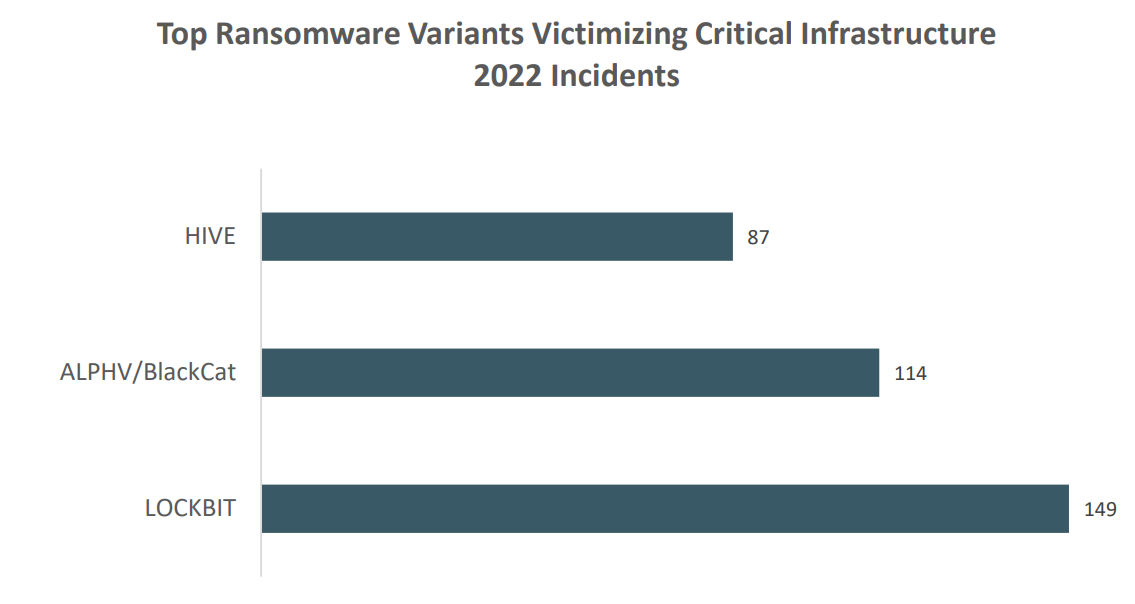
\includegraphics[width=0.75\linewidth]{rysunki/topransomwares2022.png}
     \caption{Najpopularniejsze warianty wirusów ransomware, zarejestrowane~w~trakcie incydentów mających na celu atak infrastruktury krytycznej. Należy zauważyć, że wirus \foreignquote{english}{LockBit} sprawiał najwięcej problemów. Jego wersja na system Linux nosi nazwę \foreignquote{english}{LockBit Linux-ESXi Locker }\protect\footnotemark.}
     \label{fig:enter-label}
 \end{figure}
 \footnotetext{\emph{FBI 2022 Internet Crime Report}, s. 15}

 Raport grupy \foreignquote{english}{Herjavec} donosi, że aż 70\% organizacji medycznych borykało się~z~poważnymi komplikacjami przez ataki ransomware \cite{health}.
~W~2022 roku 1 na 42 instytucje ochrony zdrowia były ofiarami tychże ataków, 74\%~z~nich to szpitale 
 \cite{etal_check_2022}.
 \begin{figure}[H]
    \centering
    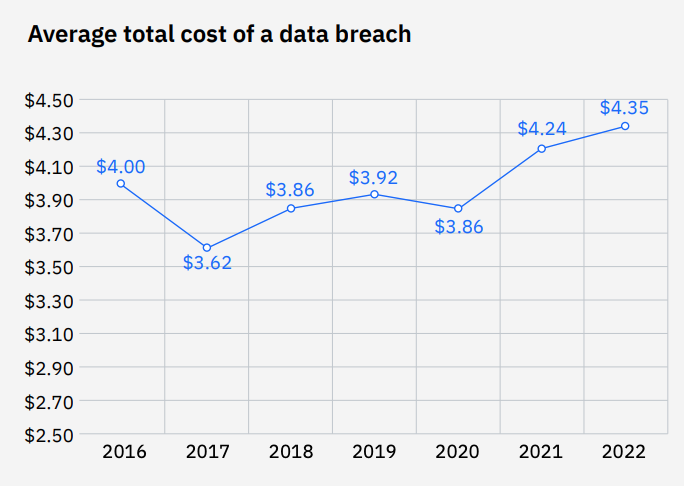
\includegraphics[width=0.7\linewidth]{rysunki/costOfDataBreach.png}
    \caption{Średni koszt naruszenia danych 2016-2022\protect\footnotemark.}
    \label{fig:enter-label}
\end{figure}
\footnotetext{\emph{Cost of~a~Data Breach
Report 2022}, figure 1, s. 9.}

~Z~danych zebranych~z~ostatnich 5 lat jednoznacznie wynika, że nieumiejętne przeciwdziałanie może zaszkodzić nie tylko finansom zaatakowanej działalności lub osoby indywidualnej, ale również stwarza zagrożenie dla zdrowia~i~życia.
 Dodatkowo, mając na uwadze średni koszt naruszenia danych~w~2023, którego globalna średnia wynosi 4,45 milionów USD \cite{petrosyan_global_cost},
 coraz więcej administratorów jest zmuszonych dywersyfikować sposoby zabezpieczania systemów. 
 \begin{figure}[H]
     \centering
     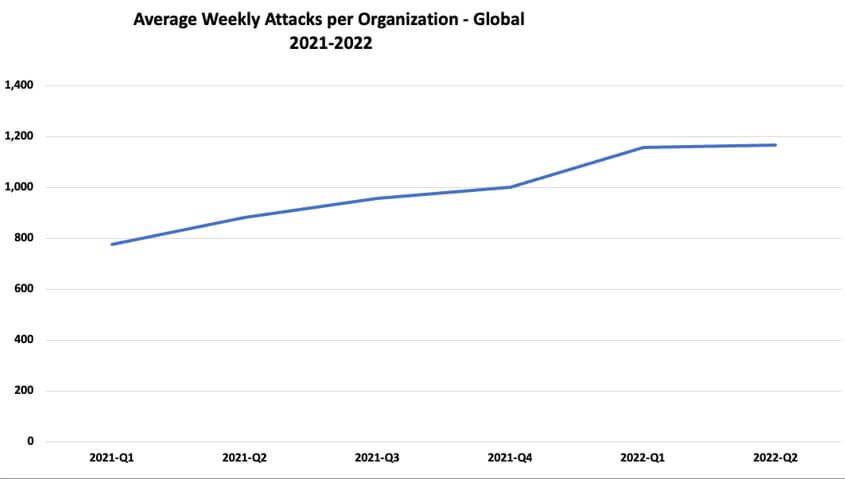
\includegraphics[width=0.75\linewidth]{rysunki/Global-Quarterly-attacks-from-Q1-2021- Q2-2022.png}
     \caption{Globalnie zgłoszone incydenty ataków ransomware per kwartał~w~roku 2022 zarejestrowanych przez Check Point Research. Organizacja spekuluje, że wzrost ataków mógł być spowodowany lukami bezpieczeństwa \foreignquote{english}{log4j} oraz cyberataków związanych~z~wojną~w~Ukrainie\protect\footnotemark.}
     \label{fig:enter-label}
 \end{figure}
\footnotetext{\emph{Check Point Research: Weekly Cyber Attacks increased by 32\% Year-Over-Year; 1 out of 40 organizations impacted by Ransomware}, figure 1.}

 Na rynku istnieje wiele popularnych rozwiązań działających prewencyjnie m.in.~w~tym rozbudowane aplikacje służące do tworzenia~i~przywracania kopii zapasowych. Należy jednak wziąć pod uwagę, że przywracanie danych nie jest prostym procesem.~W~zależności od rodzaju użytego nośnika przywracanie może doprowadzić nawet do przypadkowej utraty danych przy zniszczeniu nośnika danych~w~przypadku taśm. Jest to także proces powolny, co~w~efekcie może spowodować poniesienie większych kosztów niż wartość okupu.
 \newline
 Rozwiązaniem, które wydaje się być aktualnie najlepszym, jest możliwie jak najwcześniejsze wykrycie potencjalnego źródła ataku.~W~przypadku, gdy te czynności zawiodą, jedyną możliwością na zmniejszenie strat jest minimalizacja skutków ataku na bieżąco. Aby tego dokonać, konieczne jest wczesne wykrycie ataku.
 
\begin{figure}[H]
\centering
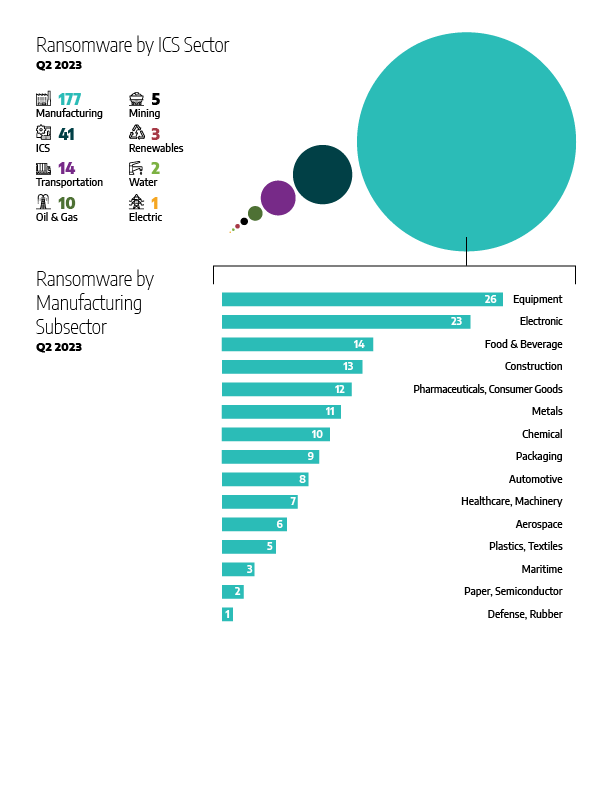
\includegraphics[width=0.6\linewidth]{rysunki/attackbysector.png}
\caption{Incydenty ransomware per sektor gospodarki\protect\footnotemark. }
\label{fig:enter-label}
\end{figure}
\footnotetext{\emph{Dragos Industrial Ransomware Attack Analysis: Q2 2023}, figure 2.}


%%%%%%%%%%%%%%%%%%%%%%%%%%%%%%%%%%%%%%%%%%%%%%%%
\section{Krótka charakterystyka ataków ransomware}
Ransomware można zdefiniować jako oprogramowanie, które blokuje atakowanemu dostęp do danych, do momentu zapłacenia okupu \cite{ransomware_us}. Prostsze ataki mogą sprowadzać się do blokady systemu bez uszkadzania plików, jednak większym zagrożeniem są tzw. \foreignquote{english}{cryptovirological attacks} \cite{502676}, czyli ataki wykorzystujące szyfrowanie danych jako formę blokady danych. Atakowany, jeśli nie posiada kopii zaszyfrowanych danych, musiałby odnaleźć klucz, którego użyto~w~szyfrowaniu. Nawet jeśli atakowany wie jakiego algorytmu użyto~w~ataku, to odnalezienie klucza jest problemem trudnym, zwłaszcza dla nowoczesnych algorytmów szyfrowania. Przykładowo, algorytm \foreignquote{english}{AES}~w~zależności od klucza występuje~w~wariantach 128,192 oraz 256-bitowych, co daje między $2^{128}$~a~$2^{256}$ możliwych wartości do sprawdzenia atakiem siłowym. 
\newline
Przy wyłudzaniu okupu, atakujący stosują również techniki zastraszenia. Przykładowo wirus \foreignquote{english}{WannaCry}, którego duża fala ataków miała miejsce~w~2017 roku \cite{czarnecki_oto_2017}, informował, że początkowy okup 300\$ per maszyna wzrośnie dwukrotnie po 3 dobach zwłoki. Po upływie tygodnia odzyskanie danych miałoby stać się niemożliwe. Atakujący wymagają, aby okup został spłacony~w~sposób trudny do wyśledzenia przez organy ścigania m.in. za pomocą kryptowalut.
\begin{figure}[H]
    \centering
    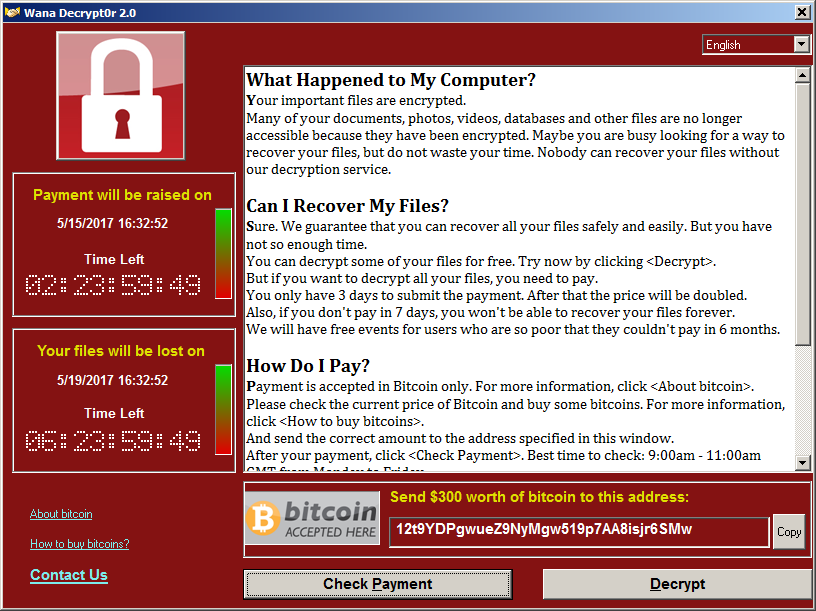
\includegraphics[width=0.8\linewidth]{rysunki/wannacry.png}
    \caption{Ekran wyświetlający się po zainfekowaniu komputera przez WannaCry. Atakujący wymaga od ofiary zapłaty Bitcoinem\protect\footnotemark.}
    \label{fig:enter-label}
\end{figure}
\footnotetext{\url{https://www.galsys.co.uk/news/wp-content/uploads/WannaCry-Pop-Up.jpg}}

Ataki ransomware, mogą także założyć blokadę powłoki systemowej lub nawet dokonać modyfikacji partycji rozruchu jak~w~przypadku wirusa RedBoot \cite{redboot}.

\begin{figure}[H]
    \centering
    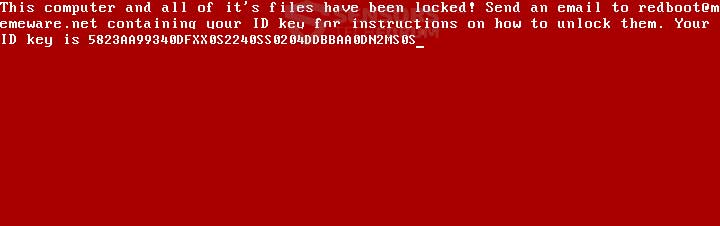
\includegraphics[width=0.95\linewidth]{rysunki/redboot.png}
    \caption{Ekran rozruchu przy infekcji wirusem RedBoot\protect\footnotemark.}
    \label{fig:enter-label}
\end{figure}
\footnotetext{\url{https://www.bleepstatic.com/images/news/ransomware/r/redboot/header.png}}

Konceptualnie \foreignquote{english}{cryptovirological attack} został przedstawiony~w~1996 roku na konferencji IEEE Security \& Privacy~\cite{yung}. Opisuje się go jako protokół pomiędzy atakowanym,~a~atakującym:

\begin{figure}[H]
    \centering
    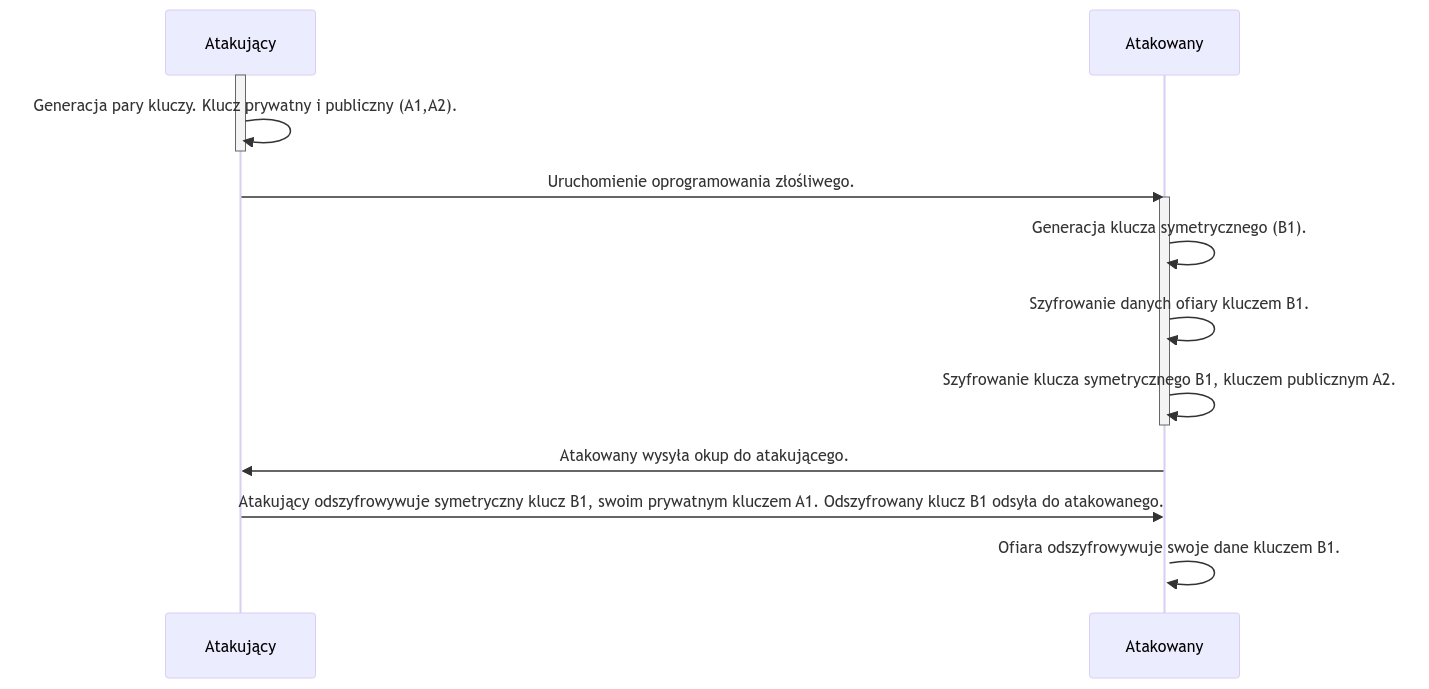
\includegraphics[width=1\linewidth]{rysunki/sequenceRansomware.png}
    \caption{Diagram sekwencji ataku ransomware.}
    \label{fig:enter-label}
\end{figure}
Generowany klucz symetryczny ma charakter losowy~i~nie pomoże~w~odszyfrowaniu danych innej ofiary. Klucz prywatny jest przechowywany wyłącznie przez atakującego. Jedyny kontakt, jaki musi być wykonany bezpośrednio przez atakującego, następuje~w~momencie kiedy zaszyfrowany klucz symetryczny jest wysyłany do atakującego,~a~następnie klucz odszyfrowany do atakowanego.
\newline
Typowymi sposobami propagacji ransomware są:
\begin{itemize}
    \item podszywanie się pod znane aplikacje czy strony internetowe,
    \item skuszenie ofiary do otworzenia niezaufanego załącznika listu elektronicznego,
    \item luki bezpieczeństwa sieci.
\end{itemize}

%%%%%%%%%%%%%%%%%%%%%%%%%%%%%%%%%%%%%%%%%%%%%%%%

% Można też wszystko pisać w jednym pliku ale będzie on duży
\chapter{Przegląd literatury}
% fragment nieużywany albo jeszcze niedodany można zakomentować
W artykule opublikowanym przez firmę Microsoft\footnote{Artykuł jest dostępny pod adresem: \url{https://www.microsoft.com/pl-pl/security/business/security-101/what-is-cybersecurity}} o tytule \enquote{Co to jest cyberbezpieczeństwo ?}, trzy z sześciu wymienionych typów zagrożenia to: 
\begin{itemize}
    \item oprogramowanie wymuszające okup,
    \item inżynieria społeczna,
    \item wyłudzanie informacji.
\end{itemize}
Atak ransomware zawiera w sobie każde z tych zagrożeń.
Oprogramowanie złośliwe wymaga od ofiary zaufania, że to co uruchamia jest nieszkodliwe. Typowo propagacja takiego malware ma miejsce poprzez tzw. 
\foreignquote{english}{phishing} czyli podszywanie się atakującego za zaufany serwis lub instytucję z którymi ofiara mogła wejść w interakcję w przeszłości. 
Aby zrozumieć zakres tych technik oraz możliwe wektory ataku, należy prześledzić ich historię.
%%%%%%%%%%%%%%%%%%%%%%%%%%%%%%%%%%%%%%%%%%%%%%%%
\section{Historia i ewolucja ataków typu ransomware}
\label{sec:his}
\subsection{Wczesna historia}
Mimo stopniowego nasilania się ataków ransomware w przeciągu ostatnich 7 lat sama idea utrudnienia
dostępu do plików pod groźbą okupu jest znana od dosyć dawna. Już w drugiej połowie lat 80-tych, w~USA,
cyberprzestępcy w zamian za odzyskanie dostępu do danych wyłudzali okup, który następnie był wysyłany drogą pocztową. Jednym z pierwszych udokumentowanych ataków wirusem ransomware był DOSowy \foreignquote{english}{AIDS trojan}~\cite{virus_1990} z 1989 roku. Autor programu — Joseph Popp — przekazywał dyskietki drogą pocztową do wybranej grupy ofiar pod przykrywką załącznika do ulotki informacyjnej na temat wirusa AIDS. Program modyfikował plik \texttt{AUTOEXEC.BAT}, z którego korzystał w celu zliczenia ilości uruchomień komputera. W momencie przekroczenia liczby 90 uruchomień szyfrował nazwy wszystkich plików na dysku \texttt{C:\/}, tym samym uniemożliwiając korzystanie z systemu.

\begin{figure}[H]
    \centering
    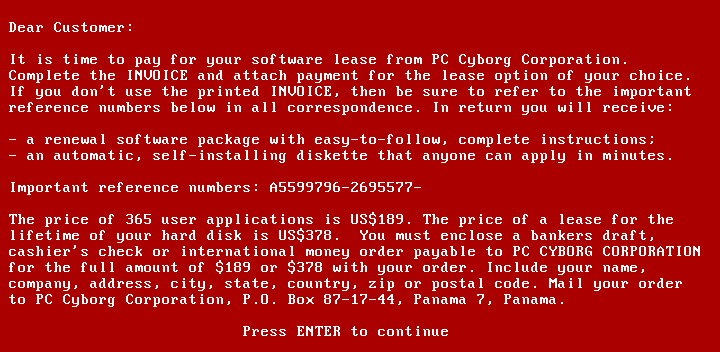
\includegraphics[width=0.6\linewidth]{rysunki/aids-trojan.png}
    \caption{Wiadomość ukazująca się po aktywacji wirusa \foreignquote{english}{AIDS trojan}\protect\footnotemark}
    \label{fig:enter-label}
\end{figure}
\footnotetext{\url{https://sophosnews.files.wordpress.com/2012/09/aids-info-demand-500.png}}

Atakujący podszywał się pod fikcyjną korporację \foreignquote{english}{PC Cyborg Corporation}, na której adres w~Panamie miał być wysyłany okup. Paczka razem z dyskietką posiadała również ulotkę z krótkim wprowadzeniem, instrukcją obsługi, a także licencją co było w tamtym czasie powszechną~i~budzącą zaufanie praktyką. 
Program nie szyfrował treści samych plików, jedynie ich nazwy. Klucz szyfrowania był kluczem symetrycznym, co sprawiało, że złamanie go mogło pomóc odblokować system, każdej ofierze borykającej się z tą samą wersją wirusa. Eliminacja tej wady była inspiracją dla pracy \foreignquote{english}{Cryptovirology: Extortion-Based Security Threats and Countermeasures}, w której przedstawiono pojęcie \foreignquote{english}{cryptovirological attack}~\cite{yung}.
\newline
Po roku 1996, w erze upowszechnienia się internetu, pojawiły się sporadyczne ataki ransomware na niewielką skalę, tym razem ulepszone o szyfrowanie hybrydowe. W latach dwutysięcznych pojawił się trudny do wykrycia \foreignquote{english}{PGPCoder}~\cite{tromer_cryptanalysis_nodate} używający 660-bitowego klucza RSA. Innym ransomware występującym w tamtym czasie był \foreignquote{english}{Archievus} ~\cite{arhiveus}, również używający klucza RSA, w wersji 1024-bitowej, którego tragiczną wadą było używanie tego samego klucza do szyfrowania każdego pliku na każdej zainfekowanej maszynie. Ataki te, aby zainfekować ofiarę, wykorzystywały phishing i~podszywały się pod zaufane strony internetowe. 
%%%%%%%%%%%%%%%%%%%%%%%%%%%%%%%%%%%%%%%%%%%%%%%%
\subsection{Historia współczesna}
Mimo historii sięgającej jeszcze lat 80 - tych, ataki ransomware nie były szczególnie powszechne w latach dwutysięcznych. Status quo został zachwiany po upowszechnieniu się kryptowalut, umożliwiających poufną~i~trudną do wyśledzenia wymianę środków między ofiarą a atakującym. Jednak uzyskanie pieniędzy od ofiar niezaznajomionych z kryptowalutami nie było proste, dopiero kantory kryptowalut dały cyberprzestępcom możliwość prostego~i~poufnego wyłudzenia środków. Pierwsza dekada XXI w. była dla cyberprzestępców czasem udoskonalania \foreignquote{english}{scareware}, czyli oprogramowania mającego wystraszyć ofiarę na tyle, żeby zapłaciła za odzyskanie dostępu do stacji, bez wyrządzania szczególnej szkody na danych. 
\newline
W 2013 roku w annały historii internetu wszedł Windowsowy wirus \foreignquote{english}{CryptoLocker}. Wykorzystywał on do szyfrowania 2048-bitową parę kluczy RSA, generowaną na osobnym serwerze, a następnie dostarczał klucz publiczny na stację ofiary w celu szyfrowania jej plików~\cite{cryptolockerfaq}. Tym samym ofiara nie miała innej możliwości odzyskania plików niż zapłacić okup wynoszący 300 USD. Wirus dostarczany był jako załącznik w liście elektronicznym oraz przez owiany złą sławą \foreignquote{english}{Gameover ZeuS botnet}~\cite{zeusbot}. Załącznik posiadał w sobie plik \texttt{.zip}, który z kolei zawierał w sobie plik \texttt{.exe}, z ikonką charakterystyczną dla pliku pdf. Atakujący wykorzystywał domyślne zachowanie Windowsa polegające na ukrywaniu rozszerzenia pliku. Następnie wirus podejmował następujące kroki:
\begin{enumerate}
    \item rozpakowywał swoje pliki w ścieżce profilu użytkownika,
    \item dodawał nową pozycję do windowsowego rejestru, który uruchamiał wirus wraz z rozruchem systemu,
    \item pobierał klucz publiczny z jednego z serwerów,
    \item wirus inicjował szyfrowanie plików na zamontowanych dyskach, w tym na dyskach sieciowych,
    \item wyświetla ekran informujący o zdarzeniu~i~możliwości opłacenia okupu w BTC do 100 godzin od zaszyfrowania.
\end{enumerate}
Po opłaceniu okupu ofiara miała możliwość pobrania programu dekodującego z załadowanym, odpowiednim kluczem prywatnym. Wirus szyfrował jedynie pliki z odpowiednimi rozszerzeniami m.in. pliki AutoCAD czy dokumenty MS Office.
\begin{figure}[H]
    \centering
    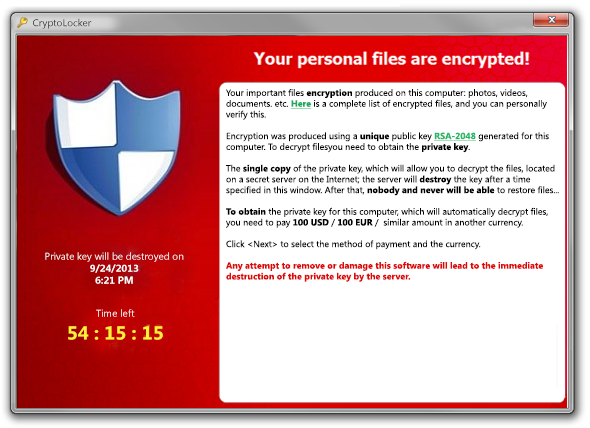
\includegraphics[width=0.75\linewidth]{rysunki/cryptolocker.png}
    \caption{Ekran wyświetlający się po zainfekowaniu komputera przez CryptoLocker\protect\footnotemark.}
    \label{fig:enter-label}
\end{figure}
\footnotetext{\url{https://grzegorzkowalik.com/wp-content/uploads/2015/05/cryptolocker.png}}
Zagrożenie tym wirusem zostało zneutralizowane w wyniku zainicjowanej przez departament sprawiedliwości USA, operacji \foreignquote{english}{Tovar}~\cite{tovar} w wyniku której udało się uzyskać dostęp do bazy danych zawierającej prywatne klucze RSA na podstawie których możliwe było odzyskanie plików.
\newline
\foreignquote{english}{CryptoLocker} był swego rodzaju kamieniem milowym w rozwoju cyberprzestępczości. Złożona natura procederu stała się normą dla ataków ransomware a wraz z coraz większą popularnością kryptowalut~i~usprawnionymi algorytmami szyfrowania asymetrycznego, ilość ataków oraz generowane przez nie straty stabilnie wzrastają aż do dnia dzisiejszego.
\newline
Aktualnie cyberprzestępcy zmienili styl ataku ze skupiającego się na infekcji jak największej ilości stacji, na tzw. \foreignquote{english}{big game hunting} (BGH)\footnote{Dokładniejszą definicję z przykładami można znaleźć pod adresem:\newline \url{https://www.malwarebytes.com/blog/news/2023/07/ransomware-making-big-money-through-big-game-hunting}}.  w dużej mierze polega na koordynacji inżynierii społecznej~i~zaprojektowania oprogramowania ransomware w sposób, który będzie najbardziej szkodliwy dla dużych organizacji. Obierana jest mniejsza ilość celów na rzecz wyższej kwoty okupu. Raport \foreignquote{english}{CrowdStrike Services} z 2023 roku donosi, że jedną najszerzej stosowanych taktyk BGH jest połączenie ransomware z groźbą upublicznienia skradzionych danych. Typowo dane zostają upubublicznione gdy minie termin zapłaty okupu. Naruszenie danych jest rozłożone w czasie~i~wykorzystuje narzędzia już dostępne na atakowanym środowisku. Dzięki temu ataki są cięższe do wykrycia\footnote{Technika ta nosi nazwę \foreignquote{english}{Living off the land}}.
Techniki zastraszenia zostały także dopracowane, aby wywołać możliwie na największą presję na ofiarach. W przypadku \foreignquote{english}{REvil} kradzione dane bywały etapowo upubliczniane, aby zmusić ofiarę do szybszego działania ~\cite{hern_ransomware_2021}.\newline
Z powodu dużej opłacalności takich ataków utworzony został model \foreignquote{english}{ransomware as a service} (RaaS), w którym klienci płacą za dokonanie ataku ransomware programem utworzonym przez inne grupy hakerskie\footnote{Wykorzystywane jest oprogramowanie utworzone przez inne osoby, podobnie jak w modelu Software as a Service.}. 
\newline
Jednym z nich jest wcześniej wymieniony \foreignquote{english}{REvil} używany przez grupę \foreignquote{english}{PINCHY SPIDER}, którego cechą rozpoznawczą jest postowanie skradzionych danych na blogu \foreignquote{english}{Happy Blog}~\cite{hern_ransomware_2021}. W 2021 roku użyto go na wysoką skalę~\cite{mcmillan_ransomware_2021} przez podatność Kaseya VSA\footnote{Kaseya VSA jest narzędziem do zarządzania infrastrukturą IT.} o identyfikatorze CVE-2021-30116~\cite{kasaya}. Atak ten można podsumować w następujących krokach:
\begin{enumerate}
    \item użycie komendy \texttt{PowerShell} do zakończenia procesów Windows Defender,
    \item podstawienie pliku wykonywalnego do katalogu instalacyjnego Windowsa,
    \item zgodnie z techniką \foreignquote{english}{Living off the land} wirus pobierał pomocnicze pliki wykonywalne~i~maskował je nazwami typowymi dla plików pomocniczych Windowsa np. \texttt{agent.exe},
    \item pobrane pliki następnie były przenoszone do odpowiednich folderów w celu załadowania ich razem z plikiem wykonywalnym \texttt{MsMpeng.exe} techniką nazywaną \foreignquote{english}{DLL sideloading}\footnote{DLL siedloading polega na załadowaniu pliku binarnego o innej treści niż oryginalna. Wykorzystuje się ją do aktywacji serwisów lub wykonywania procesów w sposób trudny do wykrycia przez użytkownika.}
    \item w momencie wywołania przez \texttt{MsMpeng.exe} serwisów, na które ma zależności, ładowany jest podłożony wcześniej plik \texttt{.dll}, a razem z nim rozpoczyna się szyfrowanie danych na maszynie,
    \item na pulpicie tworzony jest plik z instrukcją tłumaczącą jak spłacić okup w BTC na stronie ukrytej za TORem~\cite{huntresslabs_crticial_2021}.
\end{enumerate}
\begin{figure}[H]
    \centering
    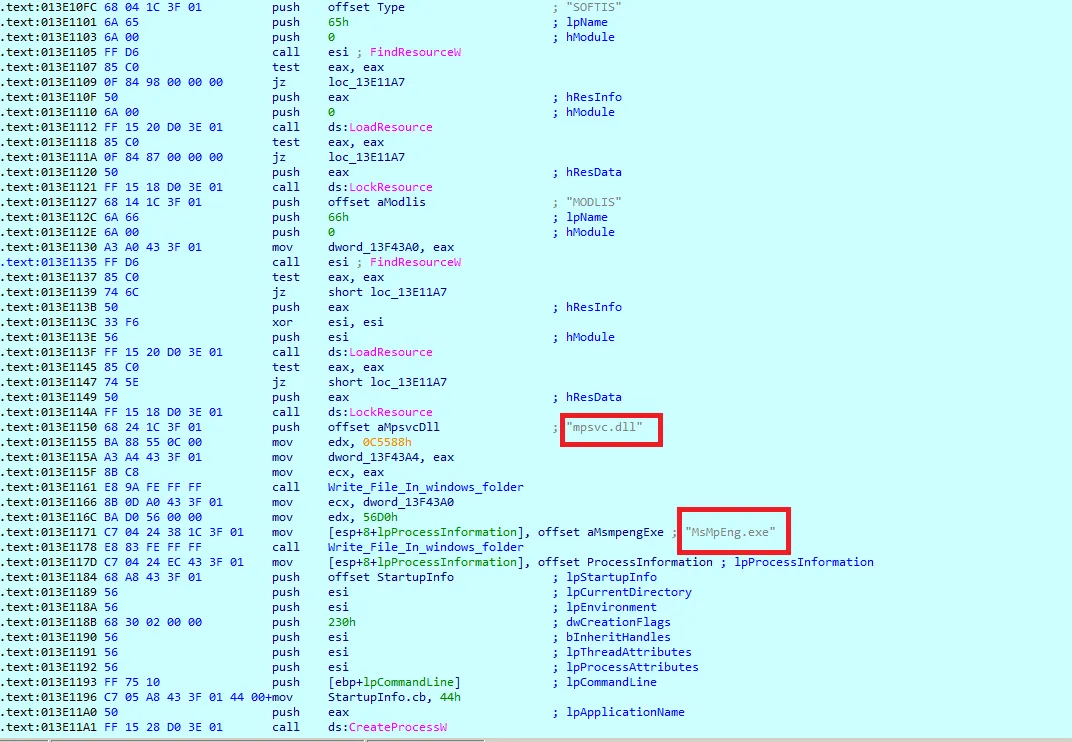
\includegraphics[width=0.8\linewidth]{rysunki/obnjdumpagenta.png}
    \caption{Miejsce w pliku binarnym \texttt{agent.exe}, w którym wywoływany jest \texttt{MsMpeng} oraz ładowany plik \texttt{.dll}\protect \footnotemark. }
    \label{fig:enter-label}
\end{figure}
\footnotetext{\url{https://ik.imagekit.io/qualys/wp-content/uploads/2021/07/Fig.-5-Write_resource_Create_process.png}}
Innym znanym RaaS jest \foreignquote{english}{DarkSide} używany przez grupę \foreignquote{english}{CARBON SPIDER}. Do niedawna skupiał się głownie na atakach maszyn Windowsowych, niedawno rozszerzając się na systemy Linux, VMware ESXi~i~vCenter~\cite{darkside}. Wirus w wersji Windowsowej obchodzi zabezpieczenia kontroli użytkownika za pomocą interfejsu \texttt{CMSTPLUA COM}\footnote{Takie obejście można dokonać programem \url{https://github.com/tijme/cmstplua-uac-bypass}}, następnie sprawdza na podstawie lokalizacji~i~języka systemu~w~celu ominięcia ataku na maszynę z jednej z byłych republik radzieckich. Program podejmuje potem następujące kroki:
\begin{enumerate}
    \item tworzy plik \texttt{LOG.<id użytkownika>.TXT} w którym przechowuje dane tymczasowe na temat progresu ataku,
    \item usuwa pliki w koszu, programy antywirusowe~i~zapewniające bezpieczeństwo oraz zamyka procesy blokujące mu dostęp do danych użytkownika,
    \item rozpoczyna szyfrowanie algorytmem \texttt{Salsa20} przy pomocy losowo wygenerowanego klucza macierzowego,
    \item klucz macierzowy jest szyfrowany zakodowanym na twardo kluczem RSA, a następnie łączony z zaszyfrowanym plikiem,
    \item pozostawia plik \texttt{README.<id użytkownika>.TXT} w którym wskazuje stronę ukrytą za TORem, na której ofiara ma dokonać płatność w BTC lub XMR.
\end{enumerate}
\begin{figure}[H]
    \centering
    
\includegraphics[width=0.75\linewidth]{rysunki/tapeta.png}
    \caption{W wyniku działania wirusa tapeta użytkownika zostaje zmieniona na taką, jak widać na obrazku\protect \footnotemark.}
    \label{fig:enter-label}
\end{figure}
\footnotetext{\url{https://staticfiles.acronis.com/images/content/5cd67c66ec1401b8e67aee9e1bb04cc4.webp}}
%%%%%%%%%%%%%%%%%%%%%%%%%%%%%%%%%%%%%%%%%%%%%%%%
\section{Istniejące techniki wykrywania i obrony przed ransomware}
\label{sec:techniques}
Niezależnie od tego czy atakujący korzysta z techniki \foreignquote{english}{living off the land} lub stara się spowodować starty w możliwie najmniejszym przedziale czasowym, 
kluczem w minimalizacji kosztów ataku ransomware najważniejsza jest szybka reakcja. Aby to osiągnąć należy podjąć inteligentną strategię, która doprowadzi do możliwie jak najwcześniejszego wykrycia ataku.
Jeśli administrator zostanie poinformowany dostatecznie wcześnie o zagrożeniu, będzie możliwa izolacja, a następnie eliminacja zagrożenia. Takie podejście w połączeniu ze 
zdyscyplinowanym harmonogramem kopii zapasowych, jest w stanie zredukować straty niemalże do zera.
\newline
Wyróżnia się trzy główne metody wykrywania ataku: poprzez sygnaturę plików, poprzez analizę nietypowego dla systemu zachowania oraz poprzez monitorowanie ruchu sieciowego~\cite{vehabovic_ransomware_2022}.
%%%%%%%%%%%%%%%%%%%%%%%%%%%%%%%%%%%%%%%%%%%%%%%%
\subsection{Wykrywanie poprzez sygnaturę plików}
Zasada działania tego typu wykrywania jest bardzo prosta. Oprogramowanie ma pewne unikalne cechy, na podstawie których wyliczana jest jego sygnatura. Do tych cech należą zakodowane na twardo nazwy domen, adresy 
IP oraz inne identyfikatory. Typowo także wykorzystywana jest wartość funkcji skrótu. Aby metoda ta mogła być skuteczna musi istnieć często aktualizowana baza danych zawierająca sygnatury wszystkich napotkanych 
typów ransomware. Niestety sposób ten jest ograniczony do wirusów napotkanych w przeszłości~i~nie jest nim możliwe wykrycie unikalnego zagrożenia.
\begin{figure}[H]
    \centering
    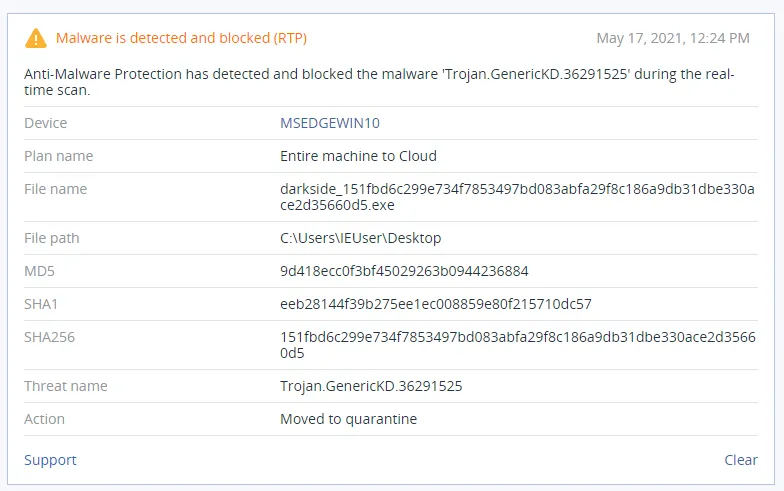
\includegraphics[width=0.65\linewidth]{rysunki/sygnatura.png}
    \caption{Tradycyjne antywirusy tak jak pokazany na obrazku Acronis, korzystają z metody wykrywania poprzez sygnaturę\protect\footnotemark.}
    \label{fig:enter-label}
\end{figure}
\footnotetext{\url{https://staticfiles.acronis.com/images/content/c110e0139779aec495bb2bd6e96ee4cd.webp}}
%%%%%%%%%%%%%%%%%%%%%%%%%%%%%%%%%%%%%%%%%%%%%%%%
\subsection{Wykrywanie poprzez analizę zachowania systemu}
\label{sec:behav}
W przeciwieństwie do wcześniej wymienionego sposobu, wykrywanie poprzez analizę zachowania system nie opiera się na sprawdzeniu treści pliku wykonywalnego, 
a na wykryciu kroków, charakterystycznych dla naruszenia bezpieczeństwa systemu. 
W przeciwieństwie do poprzedniego rozwiązania, ta metoda jest przystosowana do kontrowania techniki \foreignquote{english}{living off the land}.
Dziedzina wykrywania behawioralnego wirusów stała się m.in. obiektem badań algorytmami opartymi o sztuczną inteligencję~\cite{vehabovic_ransomware_2022}. Branych pod uwagę
może być wiele zdarzeń, z których najbardziej charakterystyczne są:
\begin{itemize}
    \item wywoływanie pewnej grupy komend powłoki systemu,
    \item pobieranie otwarto-źródłowych programów do penetracji systemów,
    \item wykorzystywanie pewnej grupy zmiennych środowiskowych jako argumenty wywołań,
    \item użycie pewnej grupy wywołań systemowych w ciągu, jedno po drugim,
    \item duży ruch w katalogach domowych użytkowników lub w \texttt{/tmp},
    \item zmiana atrybutów i właścicieli plików, katalogów czy punktów montowania dysków.
\end{itemize}
Jedną z najpowszechniejszych metod, używanym przez atakujących do powiadomienia ofiary o ataku~i~metodzie odzyskania dostępu do danych 
jest pozostawienie pliku tekstowego w miejscu łatwym do znalezienia np. w 
katalogu domowym użytkownika. Inną jest tworzenie pliku tymczasowego przechowującego 
stan zaawansowania ataku. Ze względu na to, część metod wykrywania ransomware skupia się
na wyszukiwaniu tego typu plików, na podstawie treści techniką 
\foreignquote{english}{bag-of-words}\footnote{Jest to technika przedstawienia 
tekstu w modelu nieułożonej kolekcji słów. Wykorzystuje się ją m.in. w przetwarzaniu 
języka naturalnego.} w celu odnalezienia korelacji między terminami typowymi dla 
takich dokumentów np. \foreignquote{english}{encrypted}, \foreignquote{english}{ransom}
etc.
%%%%%%%%%%%%%%%%%%%%%%%%%%%%%%%%%%%%%%%%%%%%%%%%
\subsection{Wykrywanie poprzez analizę ruchu sieciowego}
Wykrywanie poprzez analizę ruchu sieciowego polega na ograniczenia analizy behawioralnej do wyłącznie monitorowania adresatów~i~treści pakietów komunikacji sieciowej.
Szczególne zainteresowanie stanowią transfery danych do maszyn o nieznanych~i~podejrzanych adresach
oraz domenach. Zgodnie z techniką \foreignquote{english}{living off the land}, atakujący stara się
możliwe minimalizować komunikację z serwerami zewnętrznymi które mogą zostać uznane za podejrzane. Mimo to 
znakomita większość narzędzi hakerskich, jest ogólnodostępna~i~dobrze znana w branży
cyberbezpieczeństwa~i~tym samym łatwa do wykrycia~\cite{sans_secure}.  
\begin{table}[H]
    \centering
    \begin{tabular}{ll}
    \hline
    \multicolumn{1}{|l|}{Narzędzie} & \multicolumn{1}{l|}{Strona}  \\ \hline
    7zip                            & 7-zip.org                    \\
    AdFind                          & joeware.net                  \\
    Advanced IP Scanner             & advanced-ip-scanner.com      \\
    AnyDesk                         & anydesk.com                  \\
    Proces Hacker                   & processhacker.sourceforge.io \\
    rclone                          & rclone.org                   \\
    WinSCP                          & winscp.net                  
    \end{tabular}
    \caption{Tabela popularnych narzędzi wykorzystywanych w atakach ransomware\protect\footnotemark.}
\end{table}
\footnotetext{Dane pochodzą ze strony: \url{https://lots-project.com/}}
%%%%%%%%%%%%%%%%%%%%%%%%%%%%%%%%%%%%%%%%%%%%%%%%
\section{Podstawy działania systemów plików}
Struktura~i~działanie systemu plików na Linuksach jest bardzo szerokim tematem.
Na potrzeby analizy behawioralnej ataku ransomware przybliżę w tej sekcji po krótce działanie~i~
wybrane, interesujące szczegóły implementacyjne.
\subsection{Skrócony opis działania systemu plików}
Najpopularniejsze dystrybucje systemu Linux korzystają w większości z systemu plików o nazwie \texttt{ext4}.
Wprowadzony do repozytorium jądra systemowego w 2008 roku, zyskał wielkie poważanie dzięki nowoczesnej obsłudze nośników 
danych oraz ulepszeniu systemu księgowania operacji, wprodzanego w \texttt{ext3}. Księgowanie operacji w systemie plików
polega na przechowywaniu zapisów jako \emph{transakcji}. Dopiero jeśli transakcja zakończy zapisywanie na dysk, jej dane 
zostają wprowadzone na system plików~\cite{ext4}. W efekcie oznacza to, że w wypadku zaniechania działania
systemu w trakcie zapisu, transakcja zostanie cofnięta po ponownym rozruchu~i~tym samym zachowana zostanie spójność systemu plików.
\newline
Obsługa wielu rodzajów systemu plików jest możliwa dzięki istnieniu \emph{virtualnego systemu plików}. 
Jest on warstwą abstrakcji pomiędzy konkretnymi jej implmentacjami, a aplikacjami klienckimi.
Dzięki temu możliwa jest spójna~i~ujednolicona interakcja z systemem plików oraz interoperowalność między różnymi jego implementacjami~\cite{kernel}.
\begin{figure}[H]
    \centering
    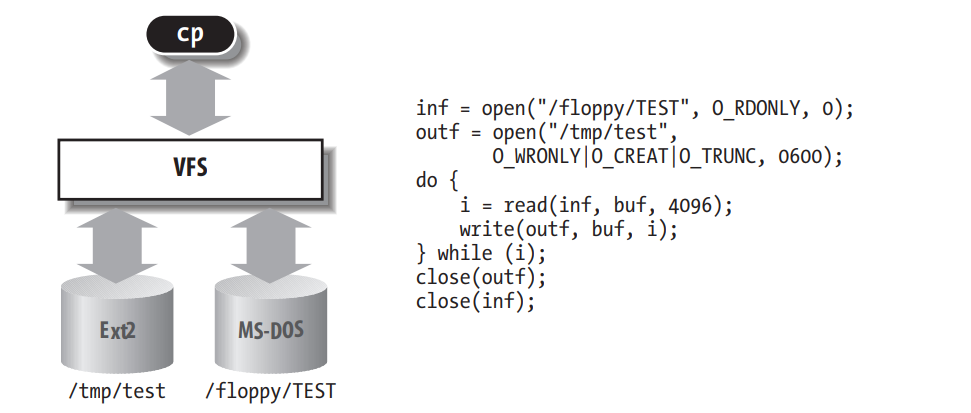
\includegraphics[width=0.9\linewidth]{rysunki/vfs.png}
    \caption{Rola wirtualnego systemu plików w operacji kopiowania\protect \footnotemark.} 
    \label{fig:enter-label}
\end{figure}
\footnotetext{\emph{Understanding Linux Kernel 3rd edition}, Figure 12-1 s. 457.}

Ogólna zasada działania wirtualnego systemu plików polegna na podmienianiu przez nią typowych wywołań systemowych
takich jak \texttt{read} lub \texttt{write} na funkcje natywne dla konkretnego systemu plików np. \texttt{ZFS} lub wcześniej wymieniony \texttt{EXT4}.
Każda implementacja musi móc przetłumaczyć swoją wewnętrzną strukturę organizacjną na model ogólny wirtualnego systemu plików~\cite{kernel}.
\begin{figure}[H]
    \centering
    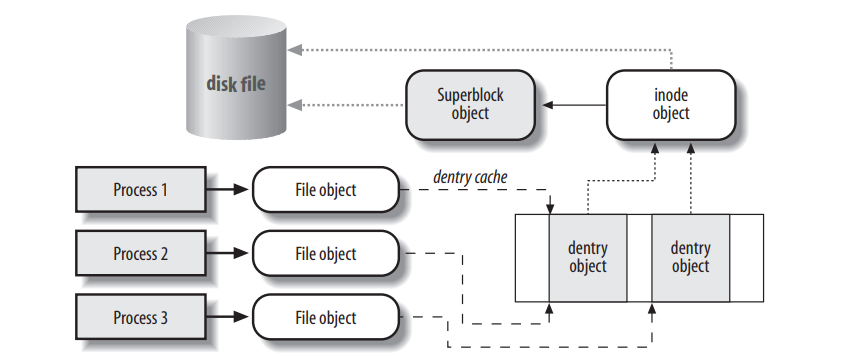
\includegraphics[width=0.9\linewidth]{rysunki/interakcjavfs.png}
    \caption{Interkacja pomiędzy procesami a objektami wirtualnego systemu plików\protect \footnotemark.} 
    \label{fig:enter-label}
\end{figure}
\footnotetext{\emph{Understanding Linux Kernel 3rd edition}, Figure 12-2 s. 460.}

Infromacje na temat interakcji pomiędzy otwartym plikiem a procesem są przechowywane~w~charakterystycznym dla procesu otwierającego plik \foreignquote{english}{file object}.
Informacje te istnieją \emph{wyłącznie}~w~pamięci jądra systemu kiedy plik jest otwarty przez proces. 
%%%%%%%%%%%%%%%%%%%%%%%%%%%%%%%%%%%%%%%%%%%%%%%%
\subsection{Monitorowanie zmian na systemie plików}
\label{sec:monitorowanie}
Jądro systemu, nie może utrzymywać zakodowanej na twardo implementacji operacji na systemie plików ze względu
na ich różnorodność. Utrzymyany jest więc indeks wskaźników do odpowienich implementacji operacji. Taka struktura komunikacji
między systemem plików a jądrem pozwala na śledzienie wywołań oprogramowaniem pośrednim. Jądro Linux zawiera w sobie dwie ciekawe
z poziomu tematu pracy impelmentacje takich \enquote{pośredników}: \foreignquote{english}{inotify subsystem} oraz \foreignquote{english}{Linux Auditing Framework}.
\subsubsection{API inotify}
\label{sec:inotify}
Podsystem inotify został stworzony z myślą o monitorowaniu oraz powiadomianiu o zmianach na dysku~\cite{love_linux_2013}. 
Jego głównym przypadkiem użycia jest automatycze aktualizowanie widoków katalogów, plików konfiuguracyjncyh, zmian
logów systemowych~i~tym podobnych. Rozwiązanie to znajduje się w kodzie źródłowym jądra Linux od sierpnia 2005 roku. Interfejs programowalny
dla tego nardzędzia zawiera się w biliotece \texttt{inotify-tools}, które zawiera w sobię również pakiet narzędzi będąch gotowymi implementacjami funkcjonalności API~\cite{biancalana_inotfy}.
\begin{lstlisting}[language=bash,
    backgroundcolor=\color{EEGold!5!white},
    caption={Przykład użycia narzędzia \texttt{inotifywait}.
    Po utworzeniu pliku ukazała się odpowiednia wiadomość},
    label={lst:helloC}]
    $ cat inotify-test.sh
    #/bin/bash
    inotifywait -m /home/user/box -e create -e moved_to |
    while read -r directory action file; do
            echo "File has been created!"
    done
    $ ./inotify-test.sh
    Setting up watches.
    Watches established.
    [1]  + 13180 suspended  ./inotify-test.sh
    $ touch box/h2
    $ fg
    [1]  + 13180 continued  ./inotify-test.sh
    File has been created!
\end{lstlisting}
Niestety rowziwązanie to nie jest perefekcyjne~i~ma swoje limity. Do nich należą:
\begin{itemize}
    \item brak wsparcia dla rekurencyjnego obserwowania ścieżek,
    \item \enquote{gubienie} niektórych wydarzeń dla starszych wersji jądra Linux,
    \item brak wsparcia niektórych wydarzeń przed wersją 5.13 jądra Linux~\cite{fanotify7},
    \item brak obserwacji dysków sieciowych.
\end{itemize}
\newpage
\subsubsection{Linux Auditing Framework}
\label{sec:auditd}
Projekt Linux Auditing Framework to podsystem wbudowany w jądro systemu Linux, którego zadaniem jest przechwytywanie,
a następnie logowanie operacji systemowych. Jego możliwości nie ograniczają się wyłacznie do 
obserwacji systemu plików. Jest on w pełni zgodny z CAPP\footnote{Controlled Access Protection Profiles to środowisko służące do niezależnej oceny, analizy i testowania produktów w celu ustanowienia wymagań bezpieczeństwa.}, a
więc może być używany jako wiarygodne źródło informacji o stanie systemu. Informacje można pobierać dzięki aplikacji
po stronie użytkownika o nazwie \texttt{auditd}. Za pomocą komponentu \texttt{auditd} możliwe jest zapisanie logów do pliku lub wysłanie ich UNIXowym gniazdkiem do innych aplikacji.
\begin{figure}[H]
    \centering
    
\includegraphics[width=0.6\linewidth]{rysunki/audit.png}
    \caption{Bardzo uproszczony diagram komponentów LAF\protect\footnotemark.}
    \label{fig:enter-label}
\end{figure}
\footnotetext{\url{https://documentation.suse.com/sles/12-SP5/html/SLES-all/cha-audit-comp.html}}

Niestety bardzo ciężko jest znaleźć informacje na temat implementacji części systemu która znajduje się w jądrze, ale 
na podstawie własnej analizy kodu zawartego w repozytorium głównym projektu\footnote{Pod adresem: \url{https://github.com/linux-audit/audit-kernel}}
, w szczególności w plikach \texttt{audit.c}, \texttt{audit\_fsnotify.c} oraz \texttt{auditsc.c} w folderze \texttt{kernel}, mogę z dużą
dozą pewności stwierdzić, że infromacje wykryte tym narzędziem są wiarygodne~i~przydatne z perspektywy tematu pracy.
W branży administracji systemami jest to narzędzie dobrze znane~i~poważane dzięki możliwościom łatwej~i~bezinwazyjnej konfiguracji.
Popularne dystrybucje serwerowe takie jak Ubuntu Server, SLES, Red Hat oraz Fedora wspierają w pełni funkcjonalności
związane z monitorowaniem systemu plików. 
%%%%%%%%%%%%%%%%%%%%%%%%%%%%%%%%%%%%%%%%%%%%%%%%
\subsection{Krótka charakterystyka plików wykonywalnych}
\label{sec:elfini}
System Linux pliki wykonywalne zapisuje~i~odczytuje w formacie \texttt{ELF} czyli 
\foreignquote{english}{Executable Linking Format}~\cite{linux_foundation_tool_nodate}.
Najciekawszym elementem tego formatu, z punktu widzenia tej pracy, jest nagłówek. Mimo, że nie zawiera tak wielu informacji co
nagłówki plików wykonywalnych na systemie Windows, warto przyjrzeć się mu aby móc zidentyfikować obecność
oprogramowania złośliwego lub narzędzia typowo wykorzystywanego podczas naruszenia bezpieczeństwa systemu.
\begin{figure}[H]
    \centering
    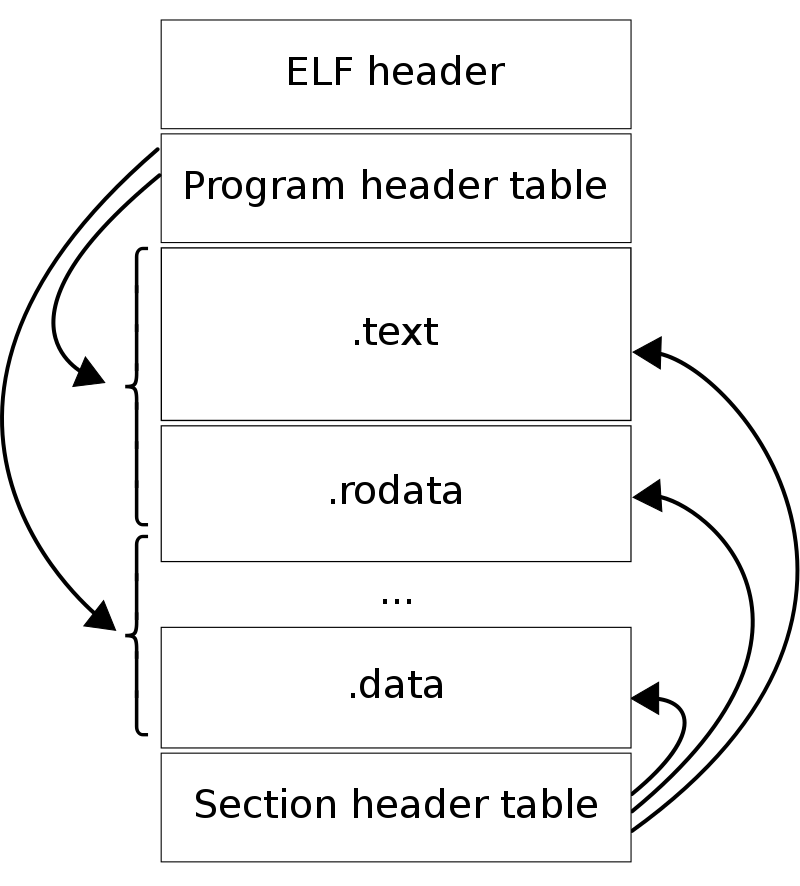
\includegraphics[width=0.45\linewidth]{rysunki/elf.png}
    \caption{Podział wewnętrzny pliku \texttt{ELF}\protect\footnotemark.}
    \label{fig:enter-label}
\end{figure}
\footnotetext{\url{https://upload.wikimedia.org/wikipedia/commons/7/77/Elf-layout--en.svg}}
W mojej opinii ciekawą sekcją jest \texttt{.note.gnu.build-id}~\cite{elfman}. Cytując
\texttt{elf(5)} Linuksowego \texttt{man pages}: \foreignquote{english}{This section is used to hold an ID that uniquely
identifies the contents of the ELF image.  Different files
with the same build ID should contain the same executable
content [...]}. Oznacza to, że można dzięki niemu \emph{zidentyfikować konkretną kompilację aplikacji}.
W przeciwieństwie do systemu Windows, gdzie typowo użytkownik pobiera już wcześniej przekompilowane pliki wykonywalne,
bardzo popularnym rozwiązaniem na Linuksach jest kompilowanie lokalnie. Wyjątkiem są zaufane repozytoria, do których dostęp
uzyskuje się przez menadżer pakietów dodawany do danej dystrybucji, np. \texttt{apt}. Mimo, że możliwa jest identyfikacja 
zawartości pliku binarnego poprzez wyliczenie jej wartości funkcji skrótu w niedługim czasie funkcją md5, identyfikator kompilacji
dla tych samych warunków kompilacji~i~zawartości kodu wykonywalnego, będzie dokładnie taki sam. Informacja ta może być wykorzystywana do
identyfikacji tego czy podejrzany plik binarny został skompilowalny lokalnie z kodu źródłowego.
\newpage
\begin{lstlisting}[language=bash,
    backgroundcolor=\color{EEGold!5!white},
    caption={Test rekompilacji aplikacji napisanej w języku Rust. Mimo ponownej kompilacji, przy braku zmiany kodu źródłowego, identyfikator pozostał ten sam.
    Można więc z dużą pewnością stwierdzić, że plik wykonywalny był skompilowalny na tej maszynie, a nie pobrany z internetu.},
    label={lst:helloC}]
    $ cargo build --release
        Finished release [optimized] target(s) in 0.13s
    $ readelf --notes target/release/linux-fs-audit | grep "Build ID"
        Build ID: ff6019887a97bedc98a8eca3267817233a13a8bc
    $ rm target/release/linux-fs-audit
    $ cargo build --release
        Finished release [optimized] target(s) in 0.04s
    $ readelf --notes target/release/linux-fs-audit | grep "Build ID"
        Build ID: ff6019887a97bedc98a8eca3267817233a13a8bc
\end{lstlisting}
%%%%%%%%%%%%%%%%%%%%%%%%%%%%%%%%%%%%%%%%%%%%%%%%
\section{Metody analizy statystyk systemu plików}
\label{sec:metody}
Wraz ze wzrostem ryzyka ataków ransomware, wzrosła też ilość prac opisujących możliwe metody wykrywania ataków
na podstawie statystyk systemowych. W tym rozdziale chciałbym wymienić~i~po krótce wytłumaczyć,~w~mojej opinii, najciekawsze z nich.
%%%%%%%%%%%%%%%%%%%%%%%%%%%%%%%%%%%%%%%%%%%%%%%%
\subsection{Analiza entropii pliku}
\label{sec:entropia}
W pracy \foreignquote{english}{Differential area analysis for ransomware
attack detection within mixed file datasets}~\cite{davies_differential_2021} przedstawiona jest 
metoda potencjalnego wykrycia tego czy plik został zaszyfrowany poprzez obliczenie entropii pliku dla różnych wielkości nagłówka.
Nagłówek~w~kontekście tej metody po prostu oznacza ilość bajtów braną pod uwagę~w~obliczaniu entropii, a niekoniecznie
twardo sprecyzowany~w~specyfikacji rodzaju pliku obszar na jego początku. Maksymalna możliwa entropia per bajt dla pliku jest równa ośmiu bitom na jeden bajt,
wartość sugerująca kompletnie losową naturę pliku. Wzór na entropię $H$~\cite{6773024} to:
$$
H(X) = - \sum_{i=1}^{n} P(x_{i})log_{2}P(x_{i})
$$
gdzie $n$ jest liczbą bajtów~w~próbce, a $P(x_{i})$ to prawdopodobieństwo wystąpienia bajtu $i$~w~strumieniu bitów.
Wyobraźmy sobie, że mamy 150 bajtowy plik który został wygenerowany losowo. Jego wykres entropi naliczonej 
od długości nagłówka $x$ będzie przypominał funkcję $log_{2}(x)$.
\begin{figure}[H]
    \centering
    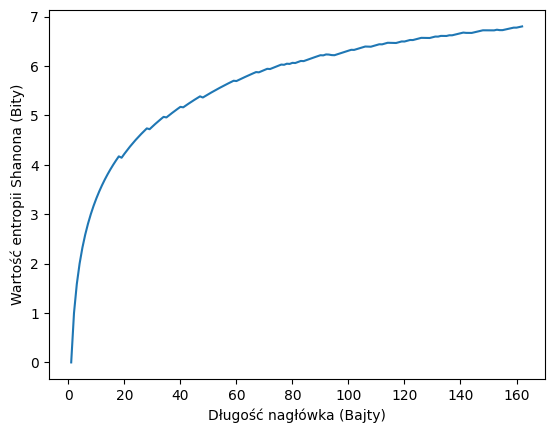
\includegraphics[width=0.65\linewidth]{rysunki/randomy.png}
    \caption{Wykres entropii od długości nagłówka dla pliku zawierającego zupełnie losowe dane.}
    \label{fig:enter-label}
\end{figure}
Dla rzeczywistych plików wartość entropii będzie rosnąć~w~mniejszym tępie, ze względu na powtarzające
się schematy~w~informacji.
\begin{figure}[H]
    \centering
    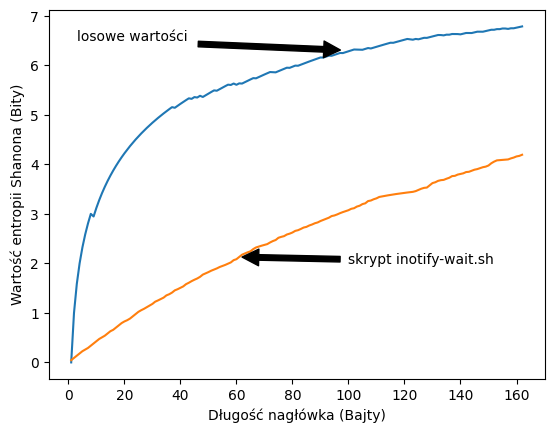
\includegraphics[width=0.65\linewidth]{rysunki/zestawienie.png}
    \caption{Zestawienie wykresów entropii od długości nagłówka. Jako plik przykładowy wybrałem skrypt~z~sekcji \hyperref[sec:monitorowanie]{Monitorowanie zmian na systemie plików}.}
    \label{fig:enter-label}
\end{figure}
Miarą tego jak duże jest prawdopodobieństwo, że plik został zaszyfrowany jest pole między tymi dwoma wykresami.
\begin{figure}[H]
    \centering
    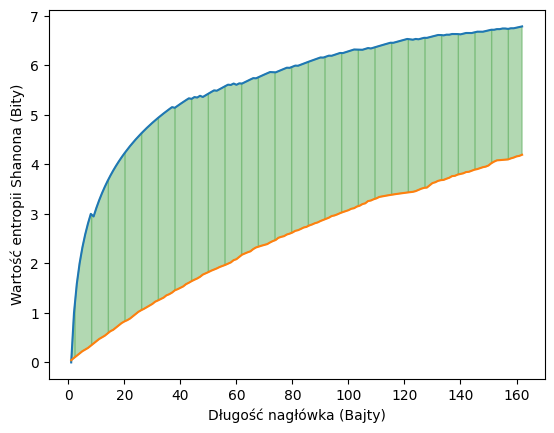
\includegraphics[width=0.7\linewidth]{rysunki/pole.png}
    \caption{Pole między wykresem losowego i rzeczywistego pliku o takich samych długościach.}
    \label{fig:enter-label}
\end{figure}
W pracy \foreignquote{english}{Differential area analysis for ransomware
attack detection within mixed file datasets}~\cite{davies_differential_2021} zasugerowane są pewne wartości klasyfikacyjne, ustalone na podstawie
dokładności wykrycia zaszyfrowanego pliku~w~zbiorach testowych.
\begin{figure}[H]
    \centering
    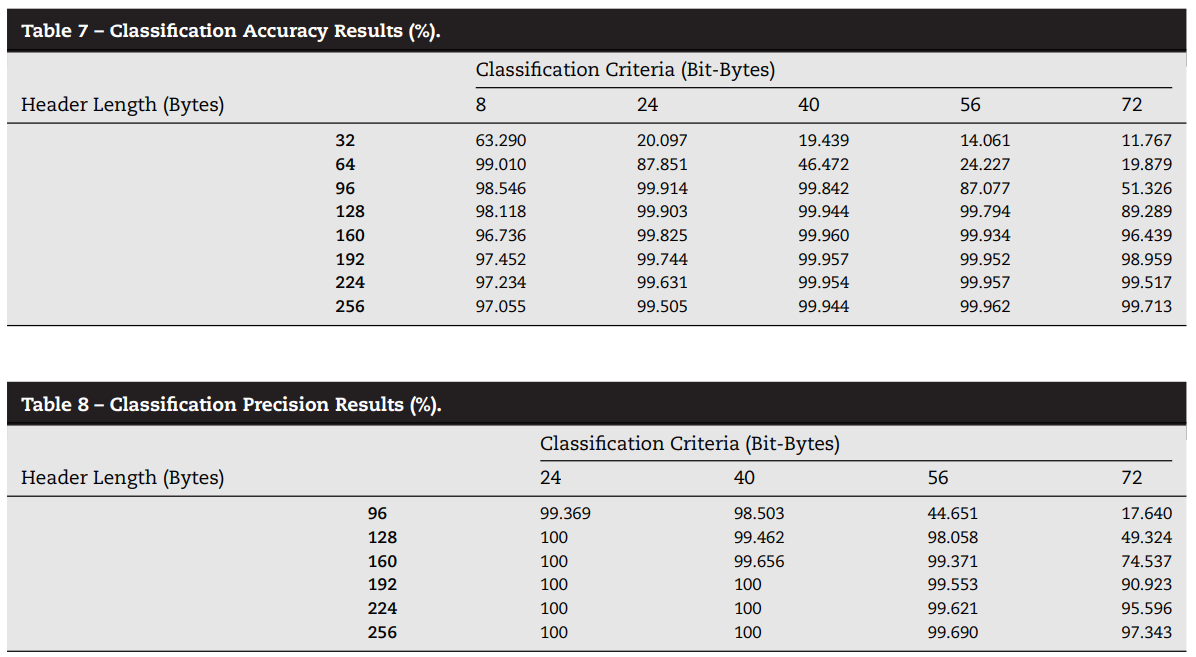
\includegraphics[width=0.85\linewidth]{rysunki/wycinek.png}
    \caption{Skuteczność dla wybranych kryteriów klasyfikacji na długość nagłówka~w~bajtach\protect\footnotemark.}
    \label{fig:enter-label}
\end{figure}
\footnotetext{\emph{Differential area analysis for ransomware
attack detection within mixed file datasets}, Table 7, Table 8, s. 11.}

Metoda ta wydaje się być bardzo obiecująca lecz jest ograniczona wymogiem wielkości pliku. Jak widać skuteczność jest lepsza dla plików o rozmiarze większym niż 32 bajty.
%%%%%%%%%%%%%%%%%%%%%%%%%%%%%%%%%%%%%%%%%%%%%%%%
\subsection{Automatyczna analiza behawioralna poprzez audyt systemu}
W pracy \foreignquote{english}{Automated Behavioral Analysis of Malware
A Case Study of WannaCry Ransomware}~\cite{8260673} opisana jest metoda identyfikacji ransomware
poprzez wyciągnięcie z logów audytu podczas rutynowego działania systemu. W przypadku tej pracy
poszukiwanie abnormalnych zachowań systemu było oparte \textbf{wyłącznie} na wiedzy o tym, że atak ma miejsce.
Aplikacja do audytowania systemu we wcześniej wymienionej pracy ma podobne możliwości do wymienionego~w~sekcji \hyperref[sec:monitorowanie]
{Monitorowanie zmian na systemie plików} Linux Auditing Framework.\newline
Przedstawiona~w~pracy metoda opera się o \foreignquote{english}{Term-Frequency-Inverse-Document-Frequency (TF-IDF)}~\cite{salton_term-weighting_1988} czyli metrykę obliczania 
wagu słów~w~oparciu o liczbę wystąpień, dostosowaną do faktu generalnie częstszego występowania niektórych słów.
Jest to metoda często wykorzysytwana~w~jako forma wydobywania informacji z tekstów m.in. \foreignquote{english}{text miningu}.
TF-IDF jest produktem dwóch statystyk: częstości występowania słowa oraz odwrotnej częstości dokumentu.
Częstotliwość występowania słowa zapisuje się wzorem:
$$
tf(t,d) = \frac{f_{t,d}}{\sum_{t'\in d}f_{t',d}}
$$
a odwrotną częstotliwość dokumentu:
$$
idf(t,D) = log \frac{N}{1 + |{d \in D : t \in d}|}
$$
gdzie słowo $t$, występujące~w~dokumencie $d$~i~wielkości zbuioru dokumentów (corpus) $N$, występuje z częstotliwością $f(t,d)$.
\newline
Niestety metoda ta nie przynosi szczególnych efektów. We wcześniej wymienionej pracy, zostały wykonane dwa eksperymenty: 
pierwszy~w~którym były wyłącznie logi z działania wirusa WannaCry oraz normalnych zachowań~w~systemie~w~osobnych dokumentach, drugi
w którym przemieszane były działania wirusa z normalnym działaniem systemu~w~tym samym dokumencie.
\begin{figure}[H]
    \centering
    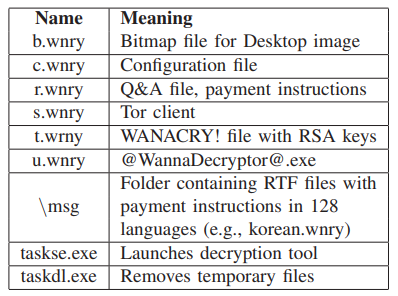
\includegraphics[width=0.3\linewidth]{rysunki/wannashit.png}
    \caption{Tabela plików tymczasowych wykorzystywanych przez wirus WannaCry\protect\footnotemark.}
    \label{fig:enter-label}
\end{figure}
\footnotetext{\emph{Automated Behavioral Analysis of Malware
A Case Study of WannaCry Ransomware}, Table I, s. 2.}

\begin{figure}[H]
    \centering
    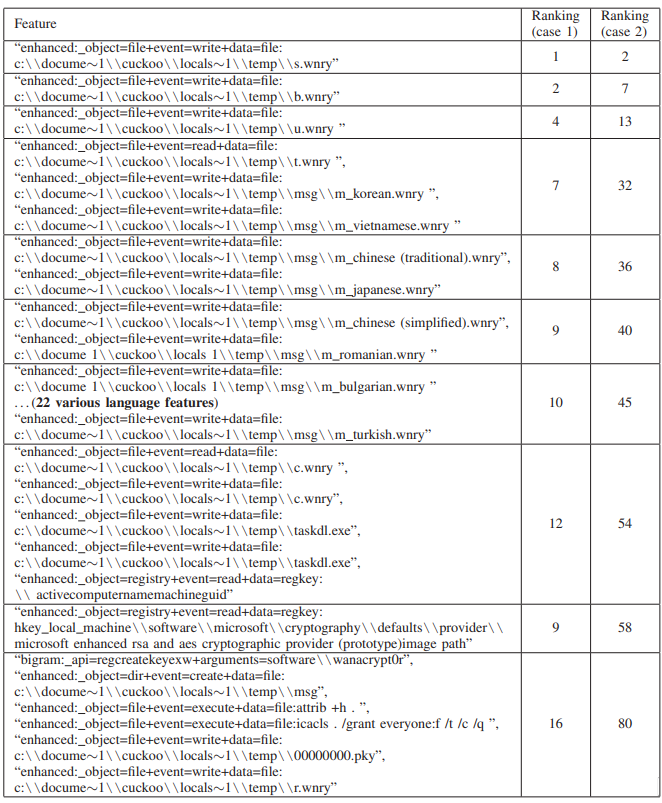
\includegraphics[width=0.85\linewidth]{rysunki/failed-exp.png}
    \caption{Tabela wyników z eksperymentu. Eksperyment pierwszy i drugi są tutaj nazwane \foreignquote{english}{case 1} i \foreignquote{english}{case 2}.
    Rankingi są wyliczone na podstawie wartości wagi TF-IDF ze wszystkich dokumentów\protect\footnotemark.}
    \label{fig:enter-label}
\end{figure}
\footnotetext{\emph{Automated Behavioral Analysis of Malware
A Case Study of WannaCry Ransomware}, Table V, s. 5.}

Jak widać z tabelki, waga informacji o działaniu ransomware znacznie zmalała po połączeniu
z logami działania systemu. Audyt systemu może być przydatny dla zaznajomionego~z~infrastrukturą
administratora lecz sama jej analiza nie jest skuteczna~w~wykrywaniu ransomware. Tym samym
informacja o dokonaniu operacji na systemie plików, sama~w~sobie nie wystarczy do wykrycia ataku.
\subsection{Analiza podobieństwa pliku wykonywalnego}
\label{sec:binaries}
Praca \foreignquote{english}{A Framework for Analyzing Ransomware using
Machine Learning}~\cite{8628743} przedstawia jako daną do przetworzenia 
przez model sztucznej inteligencji podobieńtwo cosinusowe wyliczone na 
podstawie treści wykonywalnego pliku binarnego. Podobieństwo cosinusowe
jest metodą pomiaru podobieństwa pomiędzy dwoma niezerowymi wektorami długości $n$.
Jego wartości zawierają się między zerem a jedynką. Jeśli dwa wektory mają taką samą
orientację jego wartość wynosi jeden. Dla dwóch wektorów $P$ oraz $Q$, podobieństwo 
będzie wynosić:
$$
cos(\theta) = \frac{P \cdot Q}{|P||Q|} = \frac{\sum_{i = 1}^{n} P_{i} \cdot Q_{i}}{\sqrt{\sum_{i = 1}^{n}P^{2}_{i}} \sqrt{\sum_{i = 1}^{n}Q^{2}_{i}}}
$$
W tym wypadku $P$~i~ $Q$ to dwa pliki wykonywalne, mogą to być wirusy lub zwyczajne programy codziennego użytku. Wektory te zostają utworzone na 
podstawie częstotliwości występowania instrukcji (z argumentami) kodu asemblera zdobytego z pliku binarnego, programem
\texttt{objdump}. Przykładowo dla klasycznego programu:
\begin{lstlisting}[language=C,
    backgroundcolor=\color{EEGold!5!white},
    caption={Elementarny program w C.},
    label={lst:ello}]
    #include <stdio.h>

    int main() {
        printf("Hello world!\n");
        return 0;
    }
\end{lstlisting}
do kodu asemblera będzie wyglądał w taki sposób:
\begin{lstlisting}[language=C,
    backgroundcolor=\color{EEGold!5!white},
    caption={Fragment asemblerowego kodu programu z listingu 3.},
    label={lst:ello2}]
000000000040104e <_start>:
  40104e:	f3 0f 1e fa          	endbr64
  401052:	66 90                	xchg   %ax,%ax
  401054:	31 ed                	xor    %ebp,%ebp
  401056:	49 89 d1             	mov    %rdx,%r9
  401059:	5e                   	pop    %rsi
  40105a:	48 89 e2             	mov    %rsp,%rdx
  40105d:	48 83 e4 f0          	and    $0xfffffffffffffff0,%rsp
  401061:	50                   	push   %rax
  401062:	54                   	push   %rsp
  401063:	45 31 c0             	xor    %r8d,%r8d
  401066:	31 c9                	xor    %ecx,%ecx
  401068:	48 c7 c7 46 11 40 00 	mov    $0x401146,%rdi
  40106f:	ff 15 53 2f 00 00    	call   *0x2f53(%rip) 
  401075:	f4                   	hlt
  401076:	66 2e 0f 1f 84 00 00 	cs nopw 0x0(%rax,%rax,1)
  40107d:	00 00 00 
\end{lstlisting}
Aby przedstawić jak wygląda ta metoda, spreparowałem plik zawierający wyłącznie instrukcje asemblerowe z argumentami.
Z nich wyliczyłem częstość występowania poszczególnych słów, a następnie wyliczyłem współczynnik podobieństwa ze wzoru przedstawionego wcześniej. 
Dany jest program z \hyperref[lst:ello]{listingu 3} oraz:
\begin{lstlisting}[language=C,
    backgroundcolor=\color{EEGold!5!white},
    caption={Program podobny do programu z listingu 3. Jedyną różnicą jest obecność zmiennej $i$.},
    label={lst:helloC}]
    #include <stdio.h>

    int main() {
        int i = 2;
        printf("Hello %d!\n",i);
        return 0;
    }
\end{lstlisting}
Ich podobieństwo wyliczone ze wcześniej wymienionego wzoru wynosi $cos(\theta) = 0.996289145765327$, czyli jest bardzo duże co pokrywa się z oczekiwaniami.
Jego wartość \emph{odzwierciedla} różnicę pomiędzy dwoma plikami, więc miara ta jest czuła na nawet niewielkie zmiany.
\begin{figure}[H]
    \centering
    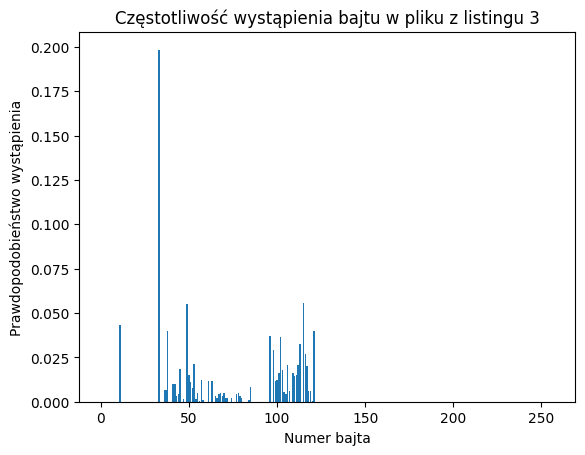
\includegraphics[width=0.69\linewidth]{rysunki/p1.png}
    \caption{Prawdopodobieństwa wystąpienia bajtów o konkretnej wartości w pliku z listingu 3.}
    \label{fig:enter-label}
\end{figure}
\begin{figure}[H]
    \centering
    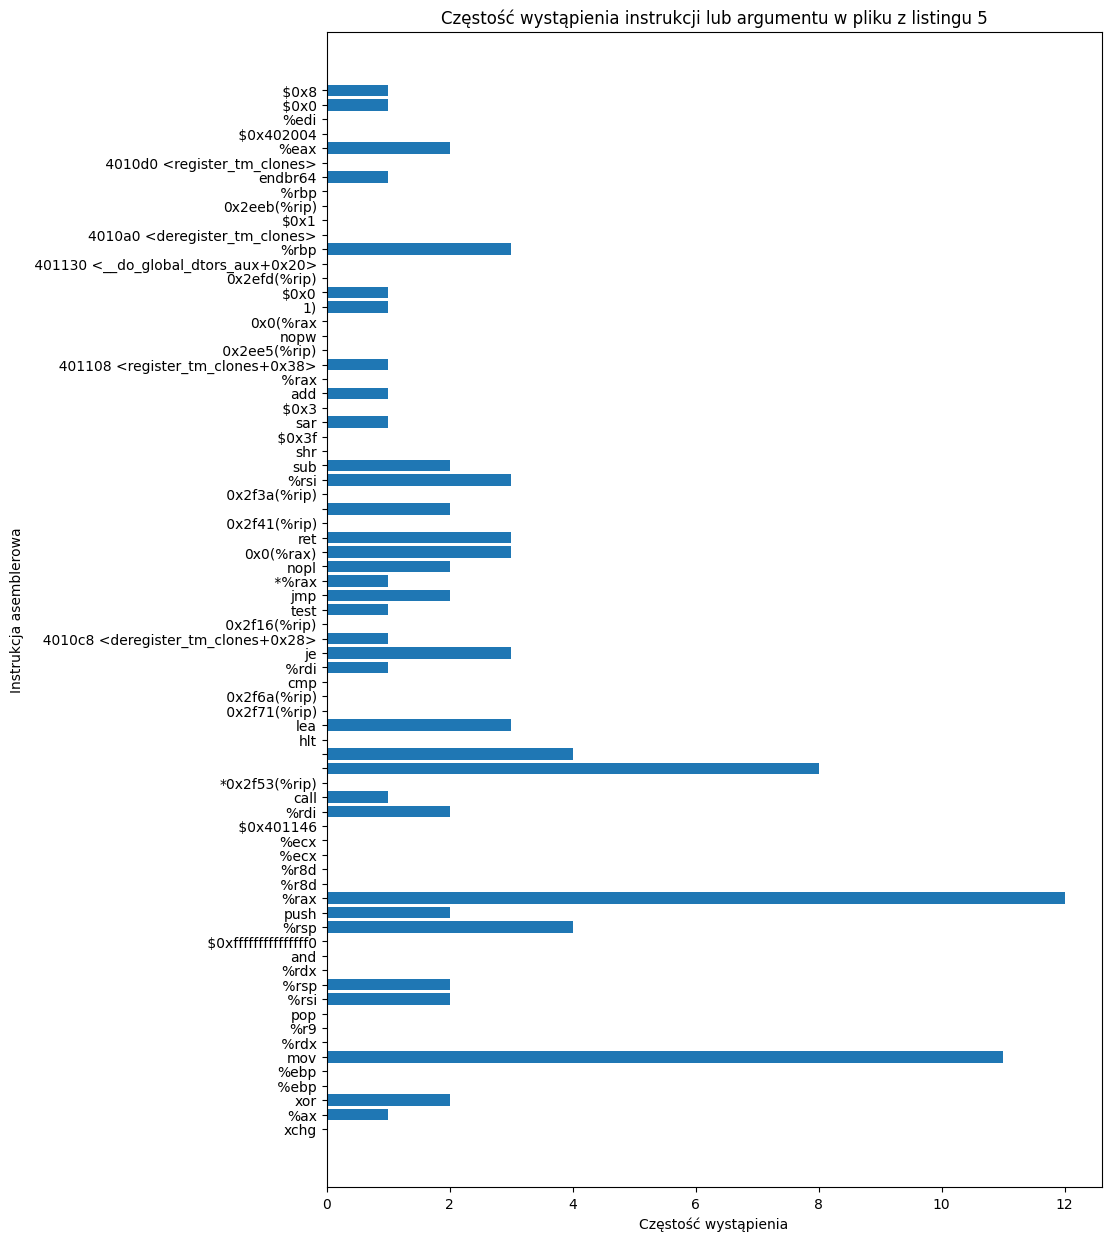
\includegraphics[width=0.69\linewidth]{rysunki/p2.png}
    \caption{Prawdopodobieństwa wystąpienia bajtów o konkretnej wartości w pliku z listingu 5.}
    \label{fig:enter-label}
\end{figure}
Jest to obiecująca metoda, która w przeciwieństwie do sprawdzania sygnatury pliku funkcją skrótu, adaptuje się do małych~i~średnich zmian w historycznie występujących zagrożeniach.
\afterpage{\blankpage}

%\input{tekst/donapisania}
\chapter{Analiza problemu}
Bedąc uzbrojonym~w~informacje wymienione we wcześniejszych rozdziałach można ułożyć model działania programu będącego celem tej pracy. Aby to jednak było możliwe należy wybrać najważniejsze informacje o maszynie, sytemie plików i odpowiednie strategie ich użycia.

\section{Charakterystyka typowych zmian~w~systemie plików podczas ataku ransomware}
\label{sec:charak}
Z informacji wymienionych~w~\hyperref[sec:monitorowanie]{Historia i ewolucja ataków typu ransomware} oraz~w~sekcji
\hyperref[sec:techniques]{Istniejące techniki wykrywania i obrony przed ransomware} można wyłuskać kilka punktów interakcji, które aktywują skan jedną~z~ metod przedstawionych~w~\hyperref[sec:techniques]{Istniejące techniki wykrywania i obrony przed ransomware}. Na potrzeby pracy proponuję: 
\begin{enumerate}
    \item przekroczenie obranej i dostatecznie wysokiej granicy wykonywanych operacji~w~ścieżce,
    \item duża ilość usuniętych a potem dodanych po sobie plików~w~obranym oknie czasowym (sugerująca zmianę nazw),
    \item powstanie plików zawierających~w~sobie słowa \enquote{README}, \enquote{LOG}, \enquote{ENCRYPTED},
    \item rutynowy skan~w~ustalonym przedziale czasowym.
\end{enumerate}
Pierwszy i drugi punkt będzie wymagał od administratora dostosowania współczynników liczbowych i tym samym dokonania korekty na własną rękę. Powodem tej konfiguracji jest indywidualna natura ruchu na danej maszynie. Na niektórych ruch będzie większy niż na innych co jest warte wzięcia pod uwagę. Punkt trzeci mimo, że jest wskaźnikiem na pierwszy rzut oka prymitywnym, jest usprawiedliwony zachowaniem dwóch najbardziej niebezpiecznych RaaS, wymienionych~w~sekcji \hyperref[sec:monitorowanie]{Historia i ewolucja ataków typu ransomware}. Rutynowy skan jest~w~dużej mierze ostateczną metodą która zostanie wykorzystana kiedy wszystkie inne zawiodą. Sama operacja skanowania będzie oparata na jednej lub kilku~z~metodach opisanych~w~sekcji \hyperref[sec:metody]{Metody analizy statystyk systemu plików}.
%%%%%%%%%%%%%%%%%%%%%%%%%%%%%%%%%%%%%%%%%%%%%%%%
\newpage
\section{Wybór odpowiednich statystyk i metryk do analizy}
\label{sec:wybor}
Aby móc przeanalizować ruch na wycześniej wymienione sposoby potrzebne będą informacje o:
% enumerate here 
\begin{itemize}
    \item czasie wystąpienia operacji~w~celu ustaleni ramki czasowej~w~której się zdarzyły,
    \item plikach zmodyfikowanach~w~ramach operacji,
    \item rodzaju operacji oraz plik wykonywalny który był jej źródłem,
    \item wywołaniu systemowym użytym~w~operacji.
\end{itemize}
Aby dokonać rzetelnego raportu dla administratora~w~moim przeczuciu należy także zawrzeć użytkownika oraz grupę będącą źródłem zaobserwowanej operacji. 
Zawarcie~w~tych statystykach nazwy wywołania systemowego ma znaczenie dla sprecyzowania jaka operacja \emph{naprawdę} została dokonana \cite{kernel}. Dany jest przykład użycia aplikacji \texttt{Visual Studio Code}: 
\begin{lstlisting}[language=bash,
    backgroundcolor=\color{EEGold!5!white},
    caption={Przykładowo używając \texttt{Visual Studio Code} niektóre operacje mogą
    sprawiać pozory, że na pliku wywołano polecenie \texttt{code} bez wiedzy co dokładnie zaszło podczas działania programu.},
    label={lst:helloC}]
    $ pidof code
    9551
    $ strace -p 9551
    strace: Process 9551 attached
    restart_syscall(<... resuming interrupted read ...>
    ) = 0
    futex(0x7ffcab93e008, FUTEX_WAKE_PRIVATE, 1) = 0
    lseek(26, 0, SEEK_SET)                  = 0
    read(26, "296974470 53709 24257 29420 0 82"..., 4095) = 38
\end{lstlisting}
W listingu wyżej można wydedukować na podstawie wiedzy o tym, że \texttt{Visual Studio Code} jest edytorem tekstowym, że otwarto plik~z~blokadą wykluczającą, wskaźnik~w~nim został przesunięty do miejsca zerowego dla pliku o deskryptorze numer dwadzieścia sześć oraz odczytano 4095 znaków od tamtego miejsca. Reasumując - odczytano plik do edycji i zablokowano do niego dostęp innym procesom.
\begin{figure}[H]
    \centering
    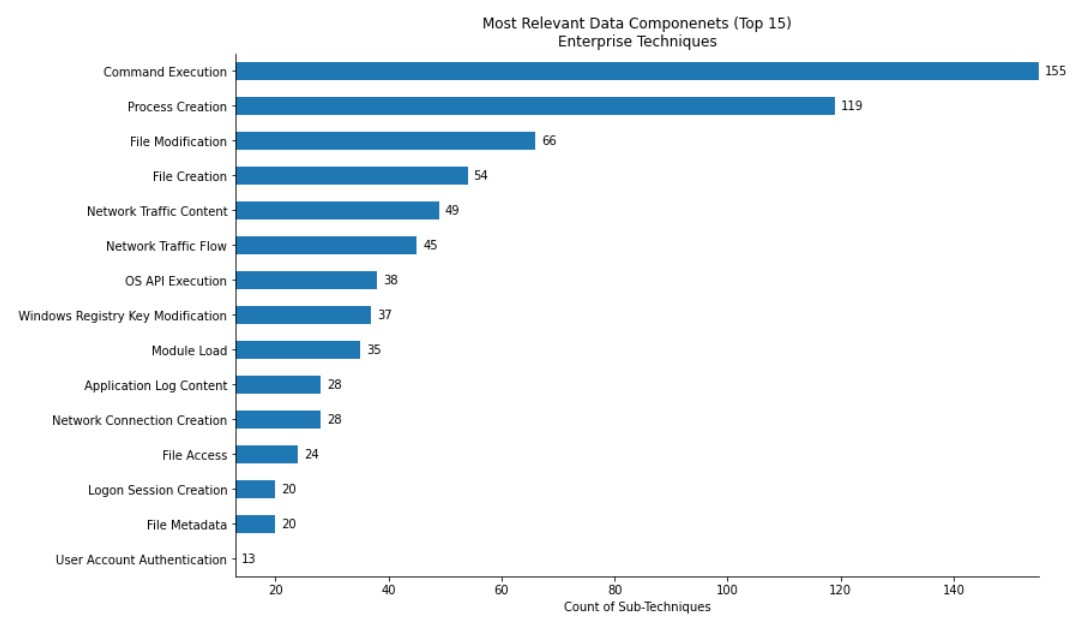
\includegraphics[width=0.5\linewidth]{rysunki/relevant_data_components.jpg}
    \caption{Najbardziej znaczące źródła danych o ataku wg. MITRE\protect\footnotemark .}
    \label{fig:enter-label}
\end{figure}
\footnotetext{\url{https://github.com/mitre-attack/attack-datasources/blob/main/docs/images/relevant_data_components.jpg}}
%%%%%%%%%%%%%%%%%%%%%%%%%%%%%%%%%%%%%%%%%%%%%%%%
\section{Potencjalne wyzwania i ograniczenia metody}
Do najciekawszych wyzwań zaproponowanego rozwiązania należą zarówno uniwersalne aspekty techniczne jak i związane~z~doborem dystrybucji i wersji jądra systemowego Linux. Rozwiązanie wykrywające operacje musi być dostatecznie rzetelne i~w~powszechnym użyciu.~W~innym wypadku kontrola systemu będzie zwyczajnie pełna luk, które same~w~sobie będą trudne do wykrycia. Efektem złego doboru roziwązania technicznego dla funckjonalności wykrywającej operacje na systemie plików może być utrata wsparcia deweloperskiego dla głównej wersji jądra systemu.
\newline
Największym wyzwaniem od strony technicznej jest utworzenie oprogramowania, którego logika wykrywania operacji na bierząco, nie będzie prowadziła do wysokiego zużycia zasobów. Zbieranie dużej ilości informacji~z~pokaźnego ciągu operacji bez wątpliwości będzie mieć wpływ na zużycie zasobów systemowych. Nie ma możliwości całkowitej eliminacji tego wpływu, można jednak podjąć kroki~w~doborze technologii~w~celu zniwelowania go. 
\newline
Mimo iż postanowiłem wybrać przypadki aktywacji funkcji skanowania ścieżki, która zazębia~z~powszechnymi scenariuszami ataku, istnieje możliwość niewystarczającego pokrycia przypadków. 
\newline
Trzeba też zaznaczyć, że dla plików skompresowanych badanie entropii ich treści może wskazywać na błędną klasyfikację~w~ramach metody przedstawionej~w~sekcji \hyperref[sec:entropia] {Analiza entropii pliku}. Nie jest to szczególnie duży problem ze względu na to, że metoda charakteryzuje się wysoką dokładnością dla plików o wielkości większej niż 32 bajty, wielkości, której przekroczenie nie jest ciężkim wyzwaniem dla plików skompresowanych. 
\newline
Metoda zaprezentowana~w~rozdziale \hyperref[sec:binaries] {Analiza podobieństwa pliku wykonywalnego} także nie jest jednoznaczną metodą wykrycia zagrożenia. Cytując abstrakt pracy \foreignquote{english}{A Framework for Analyzing Ransomware using
Machine Learning}~\cite{8628743} : \foreignquote{english}{Experimental results reported the performance
i.e. the detection accuracy of ransomware samples which varied
from 76\% to 97\% based on the ML technique used [...]}, można się spodziewać fałszywego stwierdzenia obecności ransomware~w~podobnym,~a~może i nawet rozleglejszym przedziale dokładności. 
\newline
Analizując te braki trzeba mieć na uwadze, że projektowany program ma być jednym z wielu narzędzi dla administratora ale nie ma zwalniać go z obowiązku rzetelnego analizowania potencjalnych zagrożeń na systemie. Nie ma on też być rozwiązaniem typu \enquote{wszystko w jednym}. Jego celem jest mitygacja kosztów ataku poprzez poinformowanie administratora o możliwości ataku.

\afterpage{\blankpage}
\chapter{Projekt oprogramowania i użyte rozwiązania}
\section{Specyfikacja wymagań funkcjonalnych~i~niefunkcjonalnych}
\label{sec:wymagania}
%%%%%%%%%%%%%%%%%%%%%%%%%%%%%%%%%%%%%%%%%%%%%%%%%%%%%%%%%%%%%%%%%%%
\subsection{Wymagania funkcjonalne}
\begin{table}[H]
    \begin{tabular}{|l|l|} 
    \hline
    Id: F1              & \begin{tabular}[c]{@{}l@{}}Nazwa: Identyfikacja zaszyfrowanego pliku metodą pola między \\wykresami entropii\end{tabular}                                               \\ 
    \hline
    Warunek rozpoczęcia & Skan został zainicjowany na dowolny sposób                                                                                                                              \\ 
    \hline
    Warunki zakończenia & \begin{tabular}[c]{@{}l@{}}Sukces: wynik został zwrócony\\ Porażka: wynik nie został zwrócony\end{tabular}  \\
    \hline
    \end{tabular}
\end{table}

\begin{table}[H]
    \begin{tabular}{|l|l|} 
    \hline
    Id: F2              & Nazwa: Identyfikacja ransomware poprzez podobieństwo cos                                                           \\ 
    \hline
    Warunek rozpoczęcia & \begin{tabular}[c]{@{}l@{}}Skan został zainicjowany~i~sprawdzone zostało to czy plik jest \\typu ELF\end{tabular}  \\ 
    \hline
    Warunki zakończenia & \begin{tabular}[c]{@{}l@{}}Sukces: wynik został zwrócony\\ Porażka: wynik nie został zwrócony\end{tabular}         \\
    \hline
    \end{tabular}
\end{table}

\begin{table}[H]
    \begin{tabular}{|l|l|}
    \hline
    Id: F3              & Nazwa: Analiza ruchu metodą ilości dokonanych operacji                                                                                                                                                                                           \\ \hline
    Warunek rozpoczęcia & Zainicjowana została rutynowa kontrola                                                                                                                                                                                                           \\ \hline
    Warunki zakończenia & \begin{tabular}[c]{@{}l@{}}Sukces: czas wykonania operacji mieści się~w~przedziale\\czasowym zdefiniowanym~w~konfiguracji~i~przekracza \\ ilość operacji zdefiniowaną~w~konfiguracji.\\ Porażka: niemożliwe było odczytanie danych z bazy.\end{tabular} \\ \hline
    \end{tabular}
\end{table}


\begin{table}[H]
    \begin{tabular}{|l|l|}
    \hline
    Id: F4              & Nazwa: Analiza ruchu metodą ilości zmienionych nazw plików                                                                                                                                                                                           \\ \hline
    Warunek rozpoczęcia & Zainicjowana została rutynowa kontrola                                                                                                                                                                                                           \\ \hline
    Warunki zakończenia & \begin{tabular}[c]{@{}l@{}}Sukces: czas wykonania operacji mieści się~w~przedziale\\czasowym zdefiniowanym~w~konfiguracji~i~przekracza \\ ilość operacji zdefiniowaną~w~konfiguracji.\\ Porażka: niemożliwe było odczytanie danych z bazy.\end{tabular} \\ \hline
\end{tabular}
\end{table}

\begin{table}[H]
    \begin{tabular}{|l|l|} 
    \hline
    Id: F5              & \begin{tabular}[c]{@{}l@{}}Nazwa: Analiza ruchu metodą powstania plików zawierających\\słowa kluczowe (ransom notes)\end{tabular}                                                                                                                 \\ 
    \hline
    Warunek rozpoczęcia & Zainicjowana została rutynowa kontrola                                                                                                                                                                                                            \\ 
    \hline
    Warunki zakończenia & \begin{tabular}[c]{@{}l@{}}Sukces: wykryty został plik~i~zidentyfikowany jako ransom note. \\ Porażka: niemożliwe było odczytanie danych z bazy lub plik \\ nie został wykryty mimo obecności danych o tym świadczących.\end{tabular}  \\
    \hline
    \end{tabular}
    \end{table}

\begin{table}[H]
        \begin{tabular}{|l|l|}
        \hline
        Id: F6              & Nazwa: Analiza ruchu konfigurowalnym rutynowym skanem                                                                                                                                                                                           \\ \hline
        Warunek rozpoczęcia & Zainicjowana została rutynowa kontrola                                                                                                                                                                                                           \\ \hline
        Warunki zakończenia & \begin{tabular}[c]{@{}l@{}}Sukces: skan został wykonany o czasie zdefiniowanym~w~konfiguracji. \\ Porażka: skan się nie odbył~w~sprecyzowanym czasie lub interwale.\end{tabular} \\ \hline
\end{tabular}
\end{table}

\begin{table}[H]
    \begin{tabular}{|l|l|}
    \hline
    Id: F7              & Nazwa:  Wysyłanie powiadomień na serwer \texttt{syslog}                                                                                \\ \hline
    Warunek rozpoczęcia & Zakończony został skan                                                                                                                                  \\ \hline
    Warunki zakończenia & \begin{tabular}[c]{@{}l@{}}Sukces: raport o skanie został wysłany na serwer syslog.\\ Porażka: raport nie został wysłany na serwer syslog.\end{tabular} \\ \hline
    \end{tabular}
\end{table}
%%%%%%%%%%%%%%%%%%%%%%%%%%%%%%%%%%%%%%%%%%%%%%%%%%%%%%%%%%%%%%%%%%%
\subsection{Wymagania jakościowe}
\begin{table}[H]
    \begin{tabular}{|ll|}
    \hline
    \multicolumn{1}{|l|}{ID: J1}                                                          & \begin{tabular}[c]{@{}l@{}}Nazwa:  Komponent kolekcjonowania operacji powinien być wspierany przez \\ najważniejsze dystrybucje\end{tabular}                                                        \\ \hline
    \multicolumn{2}{|l|}{Rodzaj: przenośność}                                                                                                                                                                                                                                                   \\ \hline
    \multicolumn{2}{|l|}{\begin{tabular}[c]{@{}l@{}}Opis: Aby aplikacja mogła być użyteczna dla administratorów, element odpowiadający \\ za zbieranie informacji o systemie plików musi być możliwy do użycia na popularnych\\ dystrybucjach serwerowych systemu Linux.\end{tabular}}          \\ \hline
    \multicolumn{2}{|l|}{\begin{tabular}[c]{@{}l@{}}Sposób pomiaru: Technologia wykorzystywana do zbierania informacji musi być dostępna \\ na Ubuntu 22.04.1 LTS Server, RHEL 8.8, RHEL 7.9, Open SUSE Leap 15.5 oraz SUSE \\ Linux Enterprise Server 12.\end{tabular}}                        \\ \hline
    \multicolumn{2}{|l|}{Możliwy wynik pomiaru: Funkcjonalność na danym systemie jest albo nie jest wspierana.}                                                                                                                                                                                 \\ \hline
    \multicolumn{2}{|l|}{\begin{tabular}[c]{@{}l@{}}Oczekiwanie wartości: Możliwe są tylko dwie wartości. Albo wszystkie dystrybucje wspierają \\ funkcjonalność, albo nie. Gdy chociaż jedna dystrybucja nie wspiera funkcjonalności, wymóg \\ jakościowy nie został spełniony.\end{tabular}} \\ \hline
    \end{tabular}
\end{table}
 
\begin{table}[H]
    \begin{tabular}{|ll|}
    \hline
    \multicolumn{1}{|l|}{ID: J2}                                                                                                                 & Nazwa:  Instalacja musi być bezinwazyjna                                                                                                               \\ \hline
    \multicolumn{2}{|l|}{Rodzaj: przydatność funkcjonalna}                                                                                                                                                                                                                                                \\ \hline
    \multicolumn{2}{|l|}{\begin{tabular}[c]{@{}l@{}}Opis: Instalacja nie może wymagać instalacji dodatkowych pakietów, zmiany \\ integralnych ustawienień sytemowych ani ponownego uruchamiania systemu.\end{tabular}}                                                                                  \\ \hline
    \multicolumn{2}{|l|}{\begin{tabular}[c]{@{}l@{}}Sposób pomiaru: Należy przejść przez proces instalacji~i~sprawdzić, czy \\ będzie on wymagał ponownego uruchomienia systemu lub przeładowania \\ modułów jądra systemu.\end{tabular}}                                                         \\ \hline
    \multicolumn{2}{|l|}{\begin{tabular}[c]{@{}l@{}}Możliwy wynik pomiaru: Operacja uruchomienia ponownego~i~przeładowania\\ modułów jądra systemu jest albo nie jest potrzebna przy instalacji.\end{tabular}}                                                                                            \\ \hline
    \multicolumn{2}{|l|}{\begin{tabular}[c]{@{}l@{}}Oczekiwanie wartości: Możliwe są tylko dwie wartości. Albo proces \\ wymaga naruszenia działania systemu albo nie. Jeśli wcześniej wymienione \\ działania są potrzebne~w~procesie instalacji, wymóg jakościowy nie został\\ spełniony.\end{tabular}} \\ \hline
    \end{tabular}
\end{table}

\begin{table}[H]
    \begin{tabular}{|ll|}
    \hline
    \multicolumn{1}{|l|}{ID: J3}                                                                                                                                    & Nazwa: Niskie zużycie zasobów                                                                                                                                   \\ \hline
    \multicolumn{2}{|l|}{Rodzaj: efektywność wydajnościowa}                                                                                                                                                                                                                                                                           \\ \hline
    \multicolumn{2}{|l|}{\begin{tabular}[c]{@{}l@{}}Opis: Aplikacja nie może nadwyrężać zasobów systemu~w~sposób, który\\ znacząco zmniejszałby jego możliwości obliczeniowe.\end{tabular}}                                                                                                                                           \\ \hline
    \multicolumn{2}{|l|}{\begin{tabular}[c]{@{}l@{}}Sposób pomiaru: Aplikacja powinna nie zużywać więcej niż 15\% CPU\\ dla 180 tysięcy operacji na systemie plików. Należy doprowadzić system\\ do wykonania 180 tysięcy operacji~z~pomiarem zużycia CPU.\\ Następnie powtórzyć go 10 razy~i~wyciągnąć medianę.\end{tabular}} \\ \hline
    \multicolumn{2}{|l|}{\begin{tabular}[c]{@{}l@{}}Możliwy wynik pomiaru: Zużycie mierzymy od rozpoczęcia pierwszej \\ do zakończenia ostatniej operacji. Liczy się najwyższe zużycie z całego \\ przedziału czasowego.\end{tabular}}                                                                                                \\ \hline
    \multicolumn{2}{|l|}{\begin{tabular}[c]{@{}l@{}}Oczekiwanie wartości: Mediana może przekroczyć zużycie maksymalne\\ najwyżej o 1.5 \%.~W~innym wypadku wymóg jakościowy nie został spełniony.\end{tabular}}                                                                                                                             \\ \hline
    \end{tabular}
\end{table}
%%%%%%%%%%%%%%%%%%%%%%%%%%%%%%%%%%%%%%%%%%%%%%%%%%%%%%%%%%%%%%%%%%%
\newpage
\section{Sposób zbierania~i~przetwarzania statystyk systemu plików}
Mając na uwadze wymagania z sekcji \hyperref[sec:wymagania]{Specyfikacja wymagań funkcjonalnych~i~niefunkcjonalnych}, jako silnik obserwowania operacji na systemie plików wybrałem, przedstawiony~w~\hyperref[sec:auditd]{podsekcji drugiej podrozdziału Monitorowanie zmian na systemie plików} - Linux Auditing Framework.
\begin{figure}[H]
    \centering
    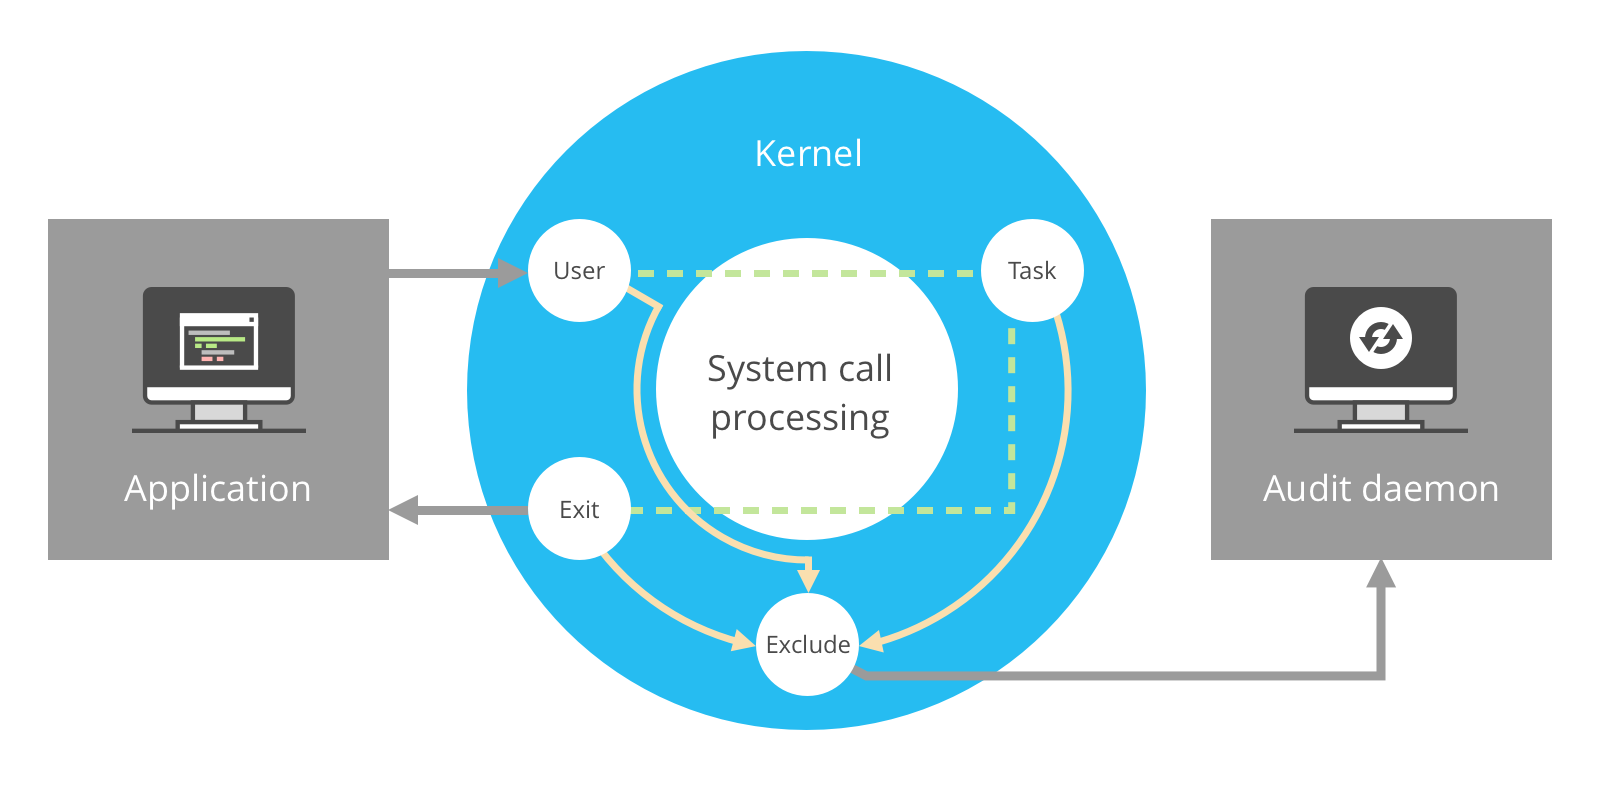
\includegraphics[width=0.9\linewidth]{rysunki/auditing.png}
    \caption{Diagram przedstawiający sekwencję działań wykonywanych~w~trakcie wykonywania operacji z równoległym audytem\protect \footnotemark.} 
    \label{fig:enter-label}
\end{figure}
\footnotetext{\url{https://selectel.ru/blog/en/2017/06/08/auditing-system-events-linux/}}

Na diagramie wyżej ukazany został bardzo ciekawy aspekt tej technologii. Mianowicie to,~że~zanim diagram stanów dla wywołania systemowego dobiegnie końca to \emph{już}, zostanie wygenerowany raport z audytu. Jest to moim zdaniem jedna z mocniejszych stron tego rozwiązania. Pozwala on~na~zniwelowanie narzutu związanego z odczytaniem informacji o operacji, tym samym zmniejszając czas reakcji wykrycia ataku. Dodatkowo jest to popularne~i~szeroko wspierne rozwiązanie o czym świadczy chociażby obecność specjalnych instrukcji obsługi dla tej technologii na stronach RedHata\footnote{\url{https://access.redhat.com/documentation/en-us/red_hat_enterprise_linux/7/html/security_guide/sec-understanding_audit_log_files}} czy OpenSuse\footnote{\url{https://doc.opensuse.org/documentation/leap/archive/42.3/security/html/book.security/cha.audit.comp.html}}.
W dużej mierze obsługa wymaga wyczytania informacji o operacji z serii logów generowanych~w~ramach raportu.
\begin{lstlisting}[language=bash,
    backgroundcolor=\color{EEGold!5!white},
    caption={Przykładowy format treści raportu z audytu. Na potrzeby estetyki prezentacji wyciąłem z niego trochę informacji.},
    label={lst:audit}]
    type=SYSCALL msg=audit(1364481363):comm="cat" exe="/bin/cat"
    type=CWD msg=audit(1364481363):  cwd="/home/shadowman"
    type=PATH msg=audit(1364481363): item=0 name="/etc/ssh/sshd_config" 
    type=PROCTITLE msg=audit(1364481363) : proctitle=6361740
\end{lstlisting}
W \hyperref[lst:audit]{listingu 7} przedstawiony jest format treści. Do najważniejszych informacji jakie można z nich wydobyć należą:
\begin{itemize}
    \item czas dokonania operacji,
    \item typ wywołania systemowego użytego~w~operacji,
    \item ścieżka do pliku wykonywalnego~w~ramach którego dokonano operacji,
    \item identyfikator użytkownika~i~jego grupy,
    \item pliki które były argumentami wywołania operacji.
\end{itemize}
Dodatkowo można sprecyzować naturę operacji~w~konfiguracji \texttt{auditd}. Przykładowo dana jest konfiguracja:
\begin{lstlisting}[language=bash,
    backgroundcolor=\color{EEGold!5!white},
    caption={Konfiguracja zasad audytowania.}
    ]
   $ sudo auditctl -a exit,always  -F dir=/dir -F perm=w -F key=WRITE
   $ sudo auditctl -a exit,always  -F dir=/dir -F perm=r -F key=READ
   $ sudo augenrules 
\end{lstlisting}
Pierwsza linijka odpowiada za wyczytywanie operacji typu \texttt{write} o kluczu \texttt{WRITE} dla ścieżki \texttt{/dir}~i~vice versa~dla~drugiej linijki z operacją \texttt{READ}. Następnie aby zmiany weszły w życie należy użyć \texttt{augenrules}. Jak więc widać konfiguracja nie jest szczególnie skomplikowana co jest również dużą zaletą tego rozwiązania. 
\newline
Ostatnią cechą wartą uwagi jest to,~że~\texttt{auditd} może zostać skonfigurowany~w~taki sposób,~że~informacje z raportów są wysyłane poprzez wybrane gniazdko UNIXowe o szczegółowo dostosowanych parametrach. Jednym z najbardziej wpływających na bezpieczeństwo atrybutów jest \texttt{direction}, który sprawia,~że~nie można żadnych danych do gniazdka wprowadzić, jedynie wyczytać. Opcja ta, nawiasem mówiąc, jest jednym z gwarantów wiarygodności informacji o systemie plików. W niżej przedstawionej konfiguracji gniazdko, na które będą kierowane informacje to \texttt{/var/run/dispatcher}. Jego atrybuty zostały ustawione w taki sposób, że użytkownik ma możliwości zapisu~i~odczytu gniazdka, grupa ma wyłącznie prawo odczytu, a inni użytkownicy nie mają żadnych do niego praw.
\begin{lstlisting}[
    backgroundcolor=\color{EEGold!5!white},
    caption={Konfiguracja opcji raportowania. 
    Więcej informacji można znaleźć na stronie RedHatowej dokumentacji \protect \footnotemark.}]
    active = yes
    direction = out
    path = builtin_af_unix
    type = builtin
    args = 0640 /var/run/dispatcher
    format = string
\end{lstlisting}
\footnotetext{\url{https://access.redhat.com/documentation/en-us/red_hat_enterprise_linux/7/html/security_guide/chap-system_auditing}}
\newpage

%%%%%%%%%%%%%%%%%%%%%%%%%%%%%%%%%%%%%%%%%%%%%%%%%%%%%%%%%%%%%%%%%%%
\section{Wybór technologii~i~narzędzi programistycznych}
\subsection{Zbieranie informacji z audytu}
Aby zbieranie informacji o systemie było możliwie szybkie~i~wydajne pamięciowo, rozważałem dwa języki - C oraz Rust. Dużą zaletą C był fakt istnienia bibliotek służących do efektywnego kolejkowania~i~parsowania informacji z audytu\footnote{\url{https://github.com/linux-audit/audit-userspace/tree/master/auparse}}. Niestety po bliższej inspekcji okazało się, że~w~implementacji kolejki następował wyciek pamięci. W związku z tym oraz prywatną chęcią bliższego zapoznania się z językiem Rust, ostatcznie wybrałem drugą opcję. Rust pozwala na stworzenie szybkiej~i~wydajnej aplikacji natywnej, jednocześnie gwarantując bezpieczeństwo pamięci. Głównie z  tego powodu wydał mi się perfekcyjnym wyborem. Aby mieć możliwość asynchronicznej obsługi wydarzeń z raportu, skorzystałem z frameworku Tokio\footnote{\url{https://tokio.rs/}}. Pozwala on na skalowalną~i~dynamiczną obsługę asynchronicznych zdarzeń~i~tym samym efektywne przetwarzanie danych. Bezpośrednim powodem użycia rozwiązania opartego na wielowątkowości było dokonanie swego rodzaju \foreignquote{english}{load balancingu} przetważanych informacji z \texttt{auditd}~w~celu mitygacji opóźnień w dostarczeniu danych wejściowych do skanowania dla dużej ilości operacji.
\begin{lstlisting}[
    backgroundcolor=\color{EEGold!5!white},
    caption={Korzystanie z możliwości tokio jest zaskakująco proste. Poza znajomością obsługi wątków w standardzie języka, wymaga ono jedynie użycia nagłówka nad funkcją \texttt{main}. Fragment kodu pochodzi z pliku \texttt{main.rs} w mojej pracy.}]
#[tokio::main]
async fn main() -> Result<(), Box<dyn std::error::Error>> {
    let configs = configure(SETTINGS_ADDRESS)?;
    simple_logger::init_with_level(match configs.log_level {
        LogSettings::Debug => Level::Debug,
        LogSettings::Info => Level::Info,
    })?;
    log::debug!("Loaded settings from: {}", SETTINGS_ADDRESS.cyan());
    // reszta kodu ...
}
\end{lstlisting}
\subsection{Logika biznesowa}
Komponent odpowiadający za logikę biznesową napisany został w Javie. Był to wybór kierowany pragmatyzmem na który złożyły się: mój osobisty stopień zaawansowania w tym języku, popularność Javy, będącej gwarancją na łatwy rozwój projektu w przyszłości~i~jej status de facto standardu aplikacji enterprise oraz międzyplatformowość.
\newline
Postanowiłem skorzystać z frameworku Spring Boot\footnote{\url{https://spring.io/projects/spring-boot}} jako naczelnego spoiwa projektu. Spring Boot oferuje wiele udogodnień przydatnych do implementacji wysokiej jakości oprogramowania. Posiada on też szeroki ekosystem tzw. starterów, czyli pakietów zależności skupiających się na różnych funkcjonalnościach np. bazach danych. Szczególnie zależało mi na możliwości korzystania z gotowej implementacji harmonogramów wywołań funkcji~i~kontenera kontekstu. 

%%%%%%%%%%%%%%%%%%%%%%%%%%%%%%%%%%%%%%%%%%%%%%%%%%%%%%%%%%%%%%%%%%%
\subsection{Baza danych}
Przy wyborze bazy danych kierowałem się założeniem, że narosnąć może potrzeba dużej ilości zapisów~i~odczytów małej ilości danych. Jako, że nie chciałem uzależniać aplikacji od dodatkowych usług, które musiałyby być serwowane na \enquote{bierząco}, zdecydowałem się na bazę SQLite. 
\newline
Technologia ta posiada wiele zalet, między innymi wymieniony wcześniej brak potrzeby serwowania danych na bazie kolejnego procesu oraz wysoką wydajność dla małej ilości zapisywanych danych. Podejmując ten wybór zainspirowałem się programem Calibre, który przechowuje informacje o ebookach w bazie SQLite-owej.

%%%%%%%%%%%%%%%%%%%%%%%%%%%%%%%%%%%%%%%%%%%%%%%%%%%%%%%%%%%%%%%%%%%

\section{Architektura aplikacji}
Najważniejsze z poziomu architektury aplikacji było~w~moim mniemaniu podzielenie logiki zbierania informacji o operacjach od logiki wykrywania zagrożenia. Celem tego zabiegu było pozostawienie możliwości łatwej zmiany technologii wysoce zależnych od implementacji, wersji czy dystrybucji systemu operacyjnego.
\begin{figure}[H]
    \centering
    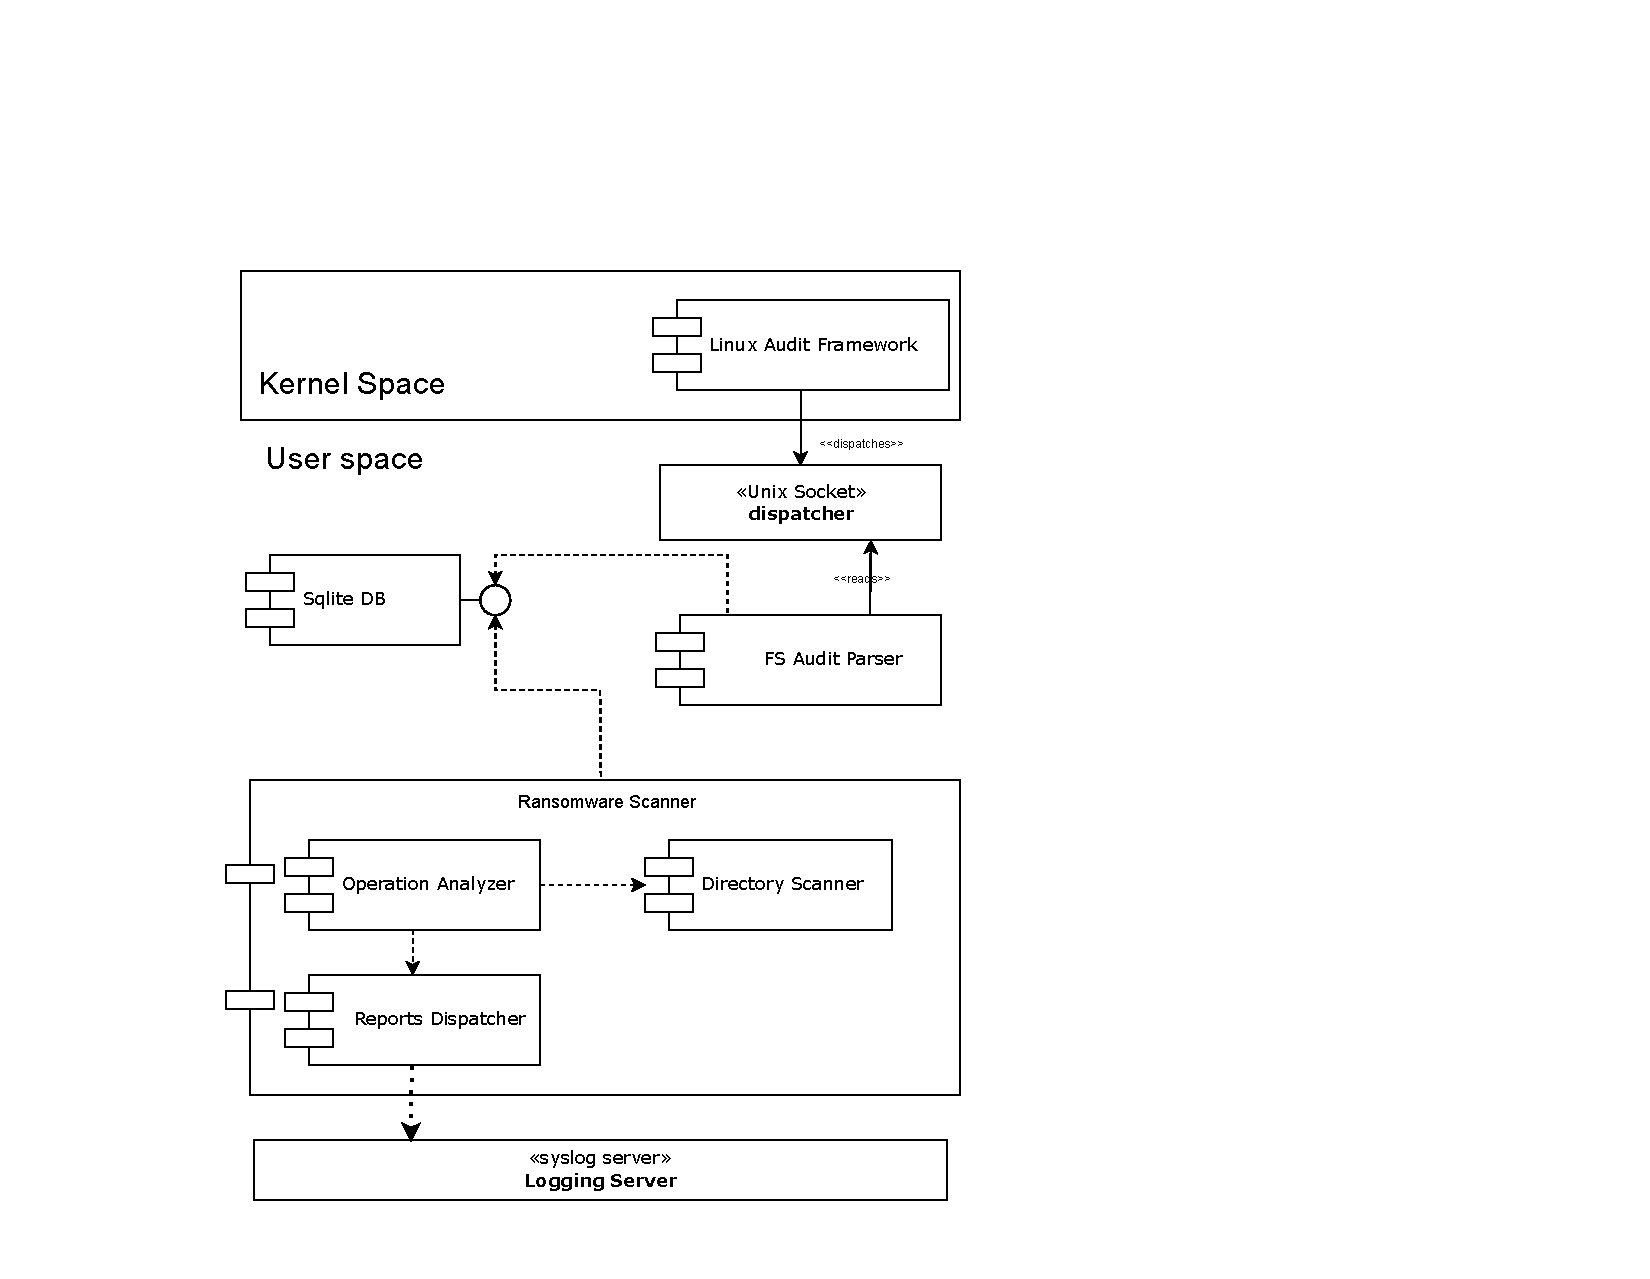
\includegraphics[width=0.52\linewidth]{rysunki/architektura-systemu.drawio.pdf}
    \caption{Diagram obrazujący zależności pomiędzy komponentami~i~źródłami informacji. Komponent \texttt{FS Audit Parser} nie komunikuje się bezpośrednio z komponentem \texttt{Ransomware Scanner}.}
    \label{fig:enter-label}
\end{figure}
Komponent FS Audit Parser odpowiada za zbieranie~i~parsowanie informacji przesyłanych przez \texttt{auditd}, będący częścią Linux Audit Framework, a następnie zapisuje je~w~bazie SQLite.
\newline
Komponent Ransomware Scanner enkapsuluje~w~sobie logikę aktywowania~i~przeprowadzania skanu~w~celu wykrycia ataku. Informacje o systemie są zbierane z bazy danych. Po przeprowadzeniu skanu wysyła on raport do serwera aplikacji \texttt{syslog}.
\newline
FS Audit Parser dokonuje wyłacznie zapisów do bazy, a Ransomware Scanner wyłącznie odczytu. Architektura aplikacji zezwala na dowolną wymianę komponentów nie będących powiązanych bezpośrednio z jej logiką biznesową jak baza danych albo metoda zczytywania wiadomości o systemie plików.

\begin{figure}[H]
    \centering
    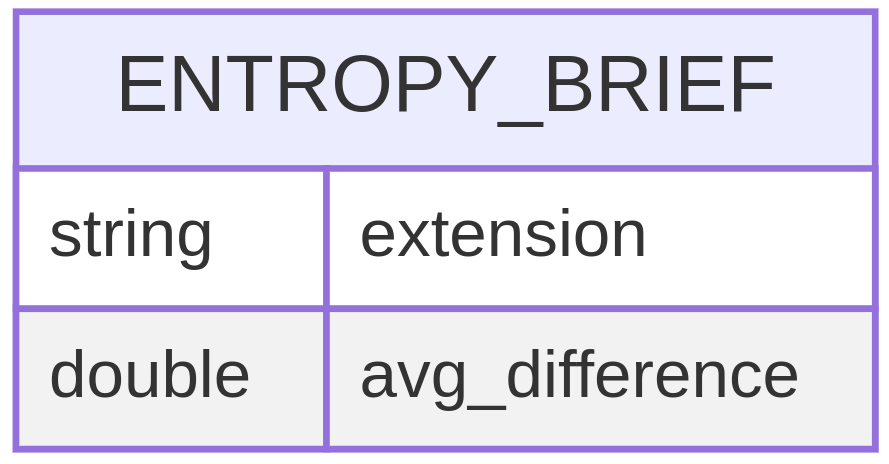
\includegraphics[width=0.3\linewidth]{rysunki/db.png}
    \caption{Schemat bazy danych.}
    \label{fig:enter-label}
\end{figure}
Projekt bazy danych jest bardzo prosty~i~oparty na podstawowych informacjach potrzebnych do implementacji logiki wykrywania ataku zdefiniowanych~w~sekcji \hyperref[sec:wybor]{Wybór odpowiednich statystyk~i~metryk do analizy}. Baza danych ma agregować funkcję przekazywania informacji między komponentami~i~zapisywaniu ich~w~celu prześledzenia danych historycznych na niewielką skalę.
\newline
Projekt architektury ze względu na silnie powiązaną dziedzinę z kontekstem technologicznym, nosi znamię pokrewnej do architektury wdrożenia. Prywatnie uważam,~że~nie jest to problemem gdyż powszechnie stosowane rozwiązania~w~cyberbezpieczeństwie \emph{nie mogą} pozwolić sobie na zupełne wyabstrachowanie swojej architektury od dziedziny technologicznej jaką mają obejmować. 
%%%%%%%%%%%%%%%%%%%%%%%%%%%%%%%%%%%%%%%%%%%%%%%%%%%%%%%%%%%%%%%%%%%
\section{Implementacja algorytmów wykrywających podejrzane działania}
%%%%%%%%%%%%%%%%%%%%%%%%%%%%%%%%%%%%%%%%%%%%%%%%%%%%%%%%%%%%%%%%%%%

\chapter{Testowanie i walidacja}
\section{Metodologia testowania}
\subsection{Warunki testowe i zastosowane środki bezpieczeństwa}
Ze względu na mój relatywny brak doświadczenia w sferze cyberbezpieczeństwa postanowiłem 
zachować możliwie największe środki ostrożności podczas wykonywania scenariuszy ataku. W szczególności tyczy się to infekcji prawdziwym wirusem ransomware.\newline
Moim stanowiskiem pracy był laptop Asus TUF Gaming FX505D~z~8 GB ramu i 512 GB pamięci NVME~z~zainstalowanym Linuksem Proxmox VE 8.1\footnote{Obraz systemu został pobrany ze strony \url{https://www.proxmox.com/en/downloads}. SHA256 obrazu wynosiło 9018a17307ad50eb9bf32a805d0917d621499363ef87b0b477332ed9f9d7dcc1.}. Proxmox jest dystrybucją specjalizującą się w zarządzaniu wirtualną infrastrukturą (na rodzaj VmWare). Posiada ona wygodny interfejs graficzny dostępny przez sieć oraz wiele udogodnień z dziedziny wirtualizacji.
\newline
Wszystkie testowane maszyny wirtualne mają zainstalowanego Ubuntu Server 22.04 LTS\footnote{\url{https://ubuntu.com/download/server}}. Każda z wirtualnych maszyn ma przydzielone 32 GB pamięci twardej, 8GB pamięci RAM oraz 8 procesorów. Jako hypervisor korzystałem~z~QEMU\footnote{\url{https://www.qemu.org/}} bez KVM\footnote{\url{https://linux-kvm.org/page/Main_Page}}.
\begin{figure}[H]
    \centering
    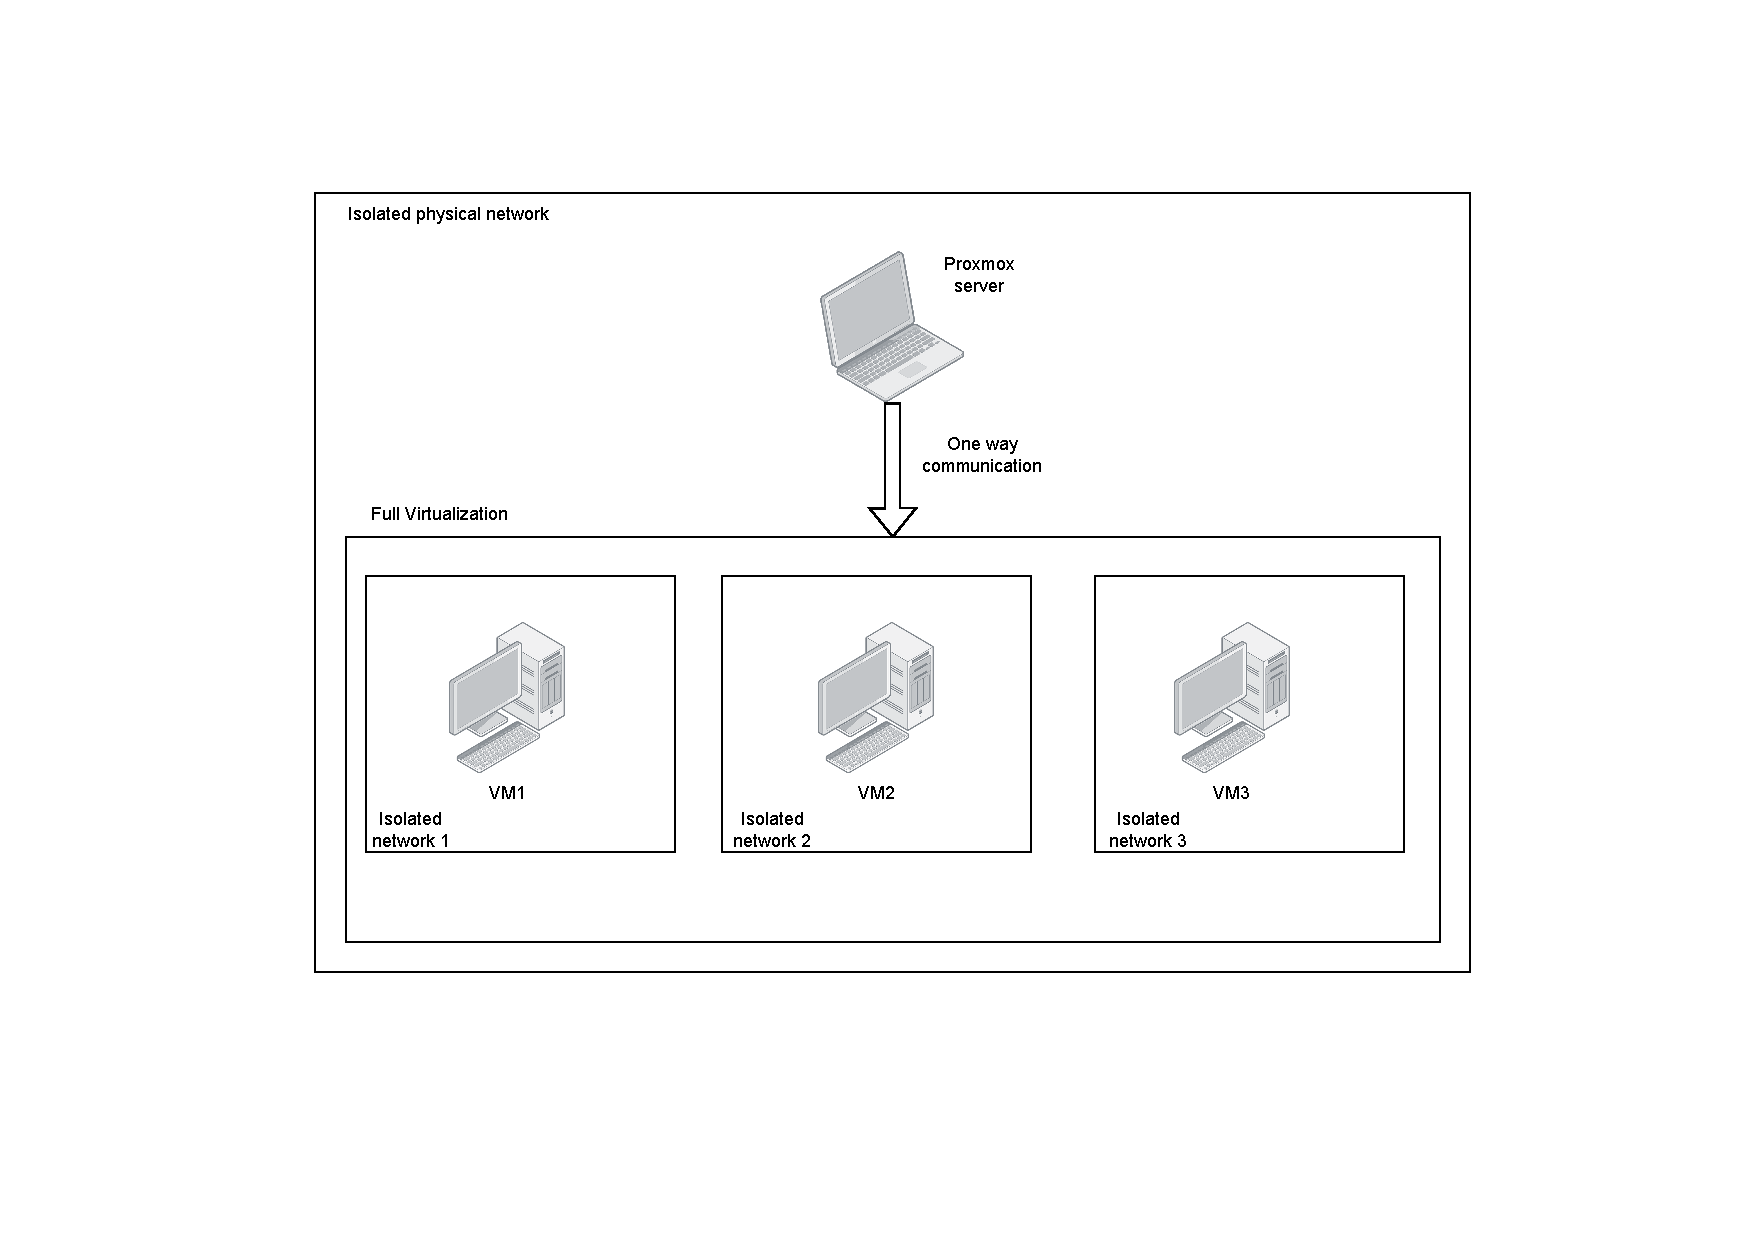
\includegraphics[width=0.45\linewidth]{rysunki/test.drawio.pdf}
    \caption{Architektura infrastruktury testowej.}
    \label{fig:enter-label}
\end{figure}
Mimo iż użycie KVM przyspieszyłoby działanie maszyn wirtualnych, postanowiłem~z~niego nie korzystać z~powodu braku konkretnych dowodów na absolutną odporność KVM switcha na oprogramowanie złośliwe. Dodatkowym środkiem bezpieczeństwa było zupełne wyizolowanie wirtualnych maszyn we własnych podsieciach na maszynie, która sama także była kompletnie fizycznie odizolowana od sieci zewnętrznych. Zasady audytu na maszynach zostały utworzone w trybie \foreignquote{english}{immutable}, tym samym nie mogły zostać zmienione bez ponownego uruchomienia systemu.

\subsection{Ustalenie metryki skuteczności rozwiązania}
Podstawowym założeniem testów była pewność odbywania się ataku podczas działania aplikacji. W tym wypadku nie ma sensu testowanie skuteczności w formie wartości dokładności wykrywania obecności ataku, gdyż jest on stałym elementem wszystkich scenariuszy. Zamiast tego postanowiłem, że skuteczność rozwiązania będzie mierzona na podstawie \emph{czasu wykrycia} od momentu rozpoczęcia ataku. Jest to miarodajna metryka naturalnie powiązanya~z~potencjalnym zakresem strat w organizacji zagrożonej ransomware.
\newline
Niestety średni czas wykrycia ataku według raportu IBMu w 2018 roku wyniósł 197 dni, a w 2019 - 207 dni~\cite{security_2019_nodate}. Aby test był możliwy do wykonania w sensownym terminie, zmuszony byłem skrócić jego czas. W związku z tym postanowiłem obrać subiektywnie wybraną miarę, umotywowaną niewielkim rozmiarem systemów użytych w testach. Mianowicie - \textbf{jeśli na 10 godzin od rozpoczęcia ataku zostanie wykryte potencjalne zagrożenie, to test został zakończony sukcesem} w przeciwnym wypadku dojdzie do porażki. W ramach testu aplikacja będzie aktywna w tle jeszcze przed rozpoczęciem ataku.
%%%%%%%%%%%%%%%%%%%%%%%%%%%%%%%%%%%%%%%%%%%%%%%%%%%%%%%%%%%%%%%%%%%%%%%%%%%%%%%%%%%%
\section{Scenariusze testowe symulujące ataki ransomware}
\subsection{Improwizowany atak~z~kompresowaniem}
Jako podstawowy scenariusz postanowiłem dokonać ataku za pomocą archiwizacji~z~szyfrowaniem w folderze~z~milionem plików. Atak miał na celu zaszyfrowanie wyłącznie plików~z~rozszerzeniem \texttt{.txt}. W tym samym miejscu obecne były również pliki o innych rozszerzeniach.
\begin{lstlisting}[language=bash,
    backgroundcolor=\color{EEGold!5!white},
    caption={Komenda użyta do wykonania "ataku".},
    label={lst:commau}]
    $ zip --encrypt files.zip *.txt
    $ rm -f *.txt
\end{lstlisting}
Warto dodać, że komenda nie wymagała przywilejów super usera. Istnieje więc możliwość wystąpienia podobnego ataku w organizacji w której doszło do wycieku danych kont pracowników bez przywilejów sudo.
\begin{lstlisting}[language=bash,
    backgroundcolor=\color{EEGold!5!white},
    caption={Fragment logów~z~komponentu zbierającego informacje o systemie plików. Będzie to jedyny tak długi fragment, który
    chciałem pokazać w celach informacyjnych.},
    label={lst:logau}]
    2023-12-17T22:33:07.316~z~INFO  [linux_fs_audit] Inserting {"user":"userA","group":"userA","executable":"/usr/bin/rm","syscall":"unlinkat","timestamp":"1702852387","key":"WRITE"}
    2023-12-17T22:33:07.351~z~INFO  [linux_fs_audit] Unix stream is readable.
    2023-12-17T22:33:07.351~z~INFO  [linux_fs_audit] Unix stream is readable.
    2023-12-17T22:33:07.351~z~WARN  [linux_fs_audit] Blocking error while reading from socket
    2023-12-17T22:33:09.762~z~INFO  [linux_fs_audit] Unix stream is readable.
    2023-12-17T22:33:09.762~z~INFO  [linux_fs_audit] Opening an Sqlite connection
    2023-12-17T22:33:09.763~z~INFO  [linux_fs_audit] Inserting {"user":"userA","group":"userA","executable":"/usr/bin/bash","syscall":"openat","timestamp":"1702852389","key":"READ"}
    2023-12-17T22:33:09.781~z~INFO  [linux_fs_audit] Opening an Sqlite connection
    2023-12-17T22:33:09.792~z~INFO  [linux_fs_audit] Unix stream is readable.
    2023-12-17T22:33:09.792~z~WARN  [linux_fs_audit] Blocking error while reading from socket
    2023-12-17T22:33:12.999~z~INFO  [linux_fs_audit] Unix stream is readable
    2023-12-17T22:33:12.999~z~INFO  [linux_fs_audit] Opening an Sqlite connection
    2023-12-17T22:33:12.999~z~INFO  [linux_fs_audit] Inserting {"user":"userA","group":"userA","executable":"/usr/bin/zip","syscall":"openat","timestamp":"1702852392","key":"WRITE"}
    2023-12-17T22:33:13.028~z~INFO  [linux_fs_audit] Opening an Sqlite connection
    2023-12-17T22:33:13.053~z~INFO  [linux_fs_audit] Unix stream is readable.
    2023-12-17T22:33:13.053~z~INFO  [linux_fs_audit] Opening an Sqlite connection
    2023-12-17T22:33:13.053~z~INFO  [linux_fs_audit] Inserting {"user":"userA","group":"userA","executable":"/usr/bin/zip","syscall":"unlink","timestamp":"1702852393","key":"WRITE"}
    2023-12-17T22:33:13.100~z~INFO  [linux_fs_audit] Opening an Sqlite connection
\end{lstlisting}
Logi~z~części aplikacji związanej ze zbieraniem informacji o systemie plików treściwie ukazują zakres działania tego komponentu. W trybie informacyjnym można zauważyć przewijanie się linijek~z~informacjami~o~odczytanych operacjach. Dodatkowo można zauważyć status odczytu~z~gniazda \texttt{auditd} oraz informacje~o~zapisie danych~o~operacji do bazy SQLite.\newpage

\begin{lstlisting}[language=bash,
    backgroundcolor=\color{EEGold!5!white},
    caption={Raport wygenerowany ze skanera, który pozwoliłem sobie delikatnie sformatować aby widać było lepiej jego treść.},
    label={lst:raportau}]
    <9>1 2023-12-18T18:11:20.485Z
    test-hostname 
    ransomware-scanner 
    - - -  
Strategy evaluations: {
    "Executable":"Low",
    "Threshold":"High",
    "Rename":"Low",
    "RansomNote":"Low"}
File risk evaluation {
    "/home/userA/box/testfile.png":"Medium",
    "/home/userA/box/h1.csv":"Low",
    "/home/userA/box/files.zip":"High",
    "/home/userA/box/h2.csv":"Low"}
\end{lstlisting}
W raporcie \enquote{z~autopsji} można zobaczyć, że jedyną metodą, która wykryła podejrzany ruch na maszynie była strategia~z~przekroczeniem ustalonej ilości operacji na jednostkę czasu. W wypadku tej maszyny było to 300 operacji na 100 ms. 
Czas wykrycia pokrył się~z~interwałem inicjalizacji analizy i wyniósł ok \textbf{167 ms}.
\newline
We fragmencie zatytułowanym \foreignquote{english}{File risk evaluation} każdy plik określony swoją absolutną ścieżką ma ustaloną wartość ewaluacji. Dla plików wykonywalnych oznacza to jak wysokie jest ryzyko tego, że program jest oprogramowaniem złośliwym. Dla wszystkich innych rodzajów plików wyznaczone jest ryzyko zaszyfrowania go. Jak widać plik \texttt{files.zip} jako jedyny został oznaczony jako plik wysokiego ryzyka bycia zaszyfrowanym.

\subsection{Atak Ransom EXX}
W drugim scenariuszu dokonałem na maszynie testowej ataku wirusem Ransom EXX. Scenariusz zakłada użycie \textbf{prawdziwego} wariantu wirusa\footnote{Na własną odpowiedzialność można go zdobyć ze strony \url{https://github.com/Gi7w0rm/RansomExx_samples_and_related_artifacts}}. Próbka którą wykorzystałem ma wartość funkcji SHA-256 równą 196eb5bfd52d4a538d4d0a801808298faadec1fc9aeb07c231add0161b416807. Wirus w tej wersji to plik wykonywalny (ELF) którego ciekawymi aspektami jest brak sekcji \texttt{.note.gnu.build-id}~o~której była mowa w sekcji \hyperref[sec:elfini]{Krótka charakterystyka plików wykonywalnych}. Postawiona przeze mnie w tamtej sekcji propozycja częściowej identyfikacji plików wykonywalnych poprzez analizę ich nagłówka miała tutaj swoje ograniczone zastosowanie. Zanim rozpocząłem atak, umieściłem w ścieżce instalacyjnej skanera wydzieloną część \texttt{.data} wirusa~z~wariantu~o~SHA-256 równym aa1ddf0c8312349be614ff43e80a262f, aby program mógł skorzystać~z~niej przy liczeniu podobieństwa cosinusowego. Atak został wywołany~z~obserwowanej ścieżki, której prefixem jest \texttt{/home}.

\begin{lstlisting}[language=bash,
    backgroundcolor=\color{EEGold!5!white},
    caption={Pierwszy raport~z~ataku Ransom EXX.},
    label={lst:raportau}]
    <9>1 2023-12-19T18:28:55.009Z
    test-hostname 
    ransomware-scanner 
    - - -  
Strategy evaluations: {
    "Rename":"Low",
    "Threshold":"Low",
    "Executable":"High",
    "RansomNote":"Low"}
File risk evaluation {
    "/home/userA/box/documentFile.txt":"Low",
    "/home/userA/box/testfile.png":"Low",
    "/home/userA/box/h1.csv":"Low",
    "/home/userA/box/h2.csv":"Low"
    "/home/maciek/box/exx196":"High"}
\end{lstlisting}
Zanim plik wykonywalny został aktywowany, jego obecność została oznaczona jako ryzykowna. Można więc powiedzieć, że test został zakończony sukcesem. Mimo to pozostawiłem maszynę do następnego dnia. Co ciekawe wg. raportu w czasie 16 godzin od rozpoczęcia ataku żaden~z~plików w \texttt{/home} nie został zaszyfrowany.
Reguły audytowania nie zostały naruszone, podobnie żaden~z~komponentów aplikacji. Dodatkowo pliki, które widać w raporcie posiadają rozszerzenia formatów będących typowym celem ataków. Jest to prawdopodobnie spowodowane powolnym działaniem wirusa.  Mimo to, podejście polegające na wykrywaniu \enquote{podejrzanych} plików i plików zaszyfrowanych znalazło tu swoje zastosowanie.
\begin{lstlisting}[language=bash,
    backgroundcolor=\color{EEGold!5!white},
    caption={Drugi raport~z~ataku Ransom EXX.},
    label={lst:raportau}]
    <9>1 2023-12-20T10:40:13.344Z
    test-hostname 
    ransomware-scanner 
    - - -  
Strategy evaluations: {
    "Rename":"Low",
    "Threshold":"Low",
    "Executable":"High",
    "RansomNote":"Low"}
File risk evaluation {
    "/home/userA/box/documentFile.txt":"Low",
    "/home/userA/box/testfile.png":"Low",
    "/home/userA/box/h1.csv":"Low",
    "/home/userA/box/h2.csv":"Low"
    "/home/maciek/box/exx196":"High"}
\end{lstlisting}
%
% Log~z~autopsji
% no bo została wykryta binarka, prawdopodobnie nie można 
%
\subsection{Atak Hive}
Hive jest wirusem występującym zarówno w wariancie Windowsowym 
jak i Linuksowym. 
Wersja Linuksowa została specjalnie stworzona pod atak infrastruktury wirtualnej, między 
innymi infekcję maszyn wirtualnych. Do ciekawych aspektów tego wirusa należy fakt napisania go w języku GO oraz to, że jego wersja Linuksowa wedle doniesień posiada wiele błędów~i~niedociągnieć. W trakcie testu napotkałem kilka~z~nich, między innymi błąd braku możliwości rozpoczęcia programu jeśli jest on wywołany wraz~z~prefixem ścieżki (bez znaczenia czy relatywnej czy absolutnej).
Próbka którą wykorzystałem ma wartość funkcji SHA-256 równą
713b699c04f21000fca981e698e1046d4595f423bd5741d712fd7e0bc358c771\footnote{Zdobyta ze strony: \url{https://bazaar.abuse.ch/sample/713b699c04f21000fca981e698e1046d4595f423bd5741d712fd7e0bc358c771/}}. Podobnie jak wirus~z~poprzedniej sekcji, występuje on w formacie ELF, lecz w przeciwieństwie do niego, posiada identyfikator kompilacji. Prawdopodobnie wynika to~z~domyślnych ustawień kompilatora GO. Również i tu wydzieliłem sekcję \texttt{.data} w celu skojarzenia podobieństwa plików wykonywalnych, ale tym razem niestety musiałem skorzystać z treści testowanego wirusa zamiast pochodnej ze względu na brak próbek. Atak został wywołany~z~obserwowanej ścieżki, której prefixem jest \texttt{/home}. Podobnie jak w porzednim scenariuszu, wirus został wykryty poprzez podobieństwo plików wykonywalnych. Z~tego powodu pozostawiłem maszynę wraz z działającym na nim wirusem na okres 10 godzin.
\begin{lstlisting}[language=bash,
    backgroundcolor=\color{EEGold!5!white},
    caption={Późniejszy raport~z~ataku Hive.},
    label={lst:raportau}]
    <9>1 2023-12-20T16:16:29.564Z
    test-hostname 
    ransomware-scanner 
    - - -  
Strategy evaluations: {
    "Rename":"Low",
    "Threshold":"Low",
    "Executable":"High",
    "RansomNote":"High"}
File risk evaluation {
    "/home/userA/box/HOW-TO-DECRYPT.txt": "High",
    "/home/userA/box/documentFile.txt":"Low",
    "/home/userA/box/testfile.png":"Low",
    "/home/userA/box/h1.csv":"Low",
    "/home/userA/box/h2.csv":"Low"
    "/home/maciek/box/hive":"High"}
\end{lstlisting}
Wyniki były zaskakujące. Według raportu, żaden~z~plików nie został zaszyfrowany. W obserwowanym folderze pojawił się plik \foreignquote{english}{HOW-TO-DECRYPT.txt} oceniony metodą wykrywania wiadomości~o~okupie jako niebezpieczny. W raporcie można także wyczytać, że wirus został wykryty metodą podobieństwa cosinusowego~o~czym wspomniałem wcześniej.\newpage
\begin{lstlisting}[
    backgroundcolor=\color{EEGold!5!white},
    caption={Fragment wiadomości~o~okupie. Ze względów bezpieczeństwa usunąłem wszelkie linki, loginy i hasła~z~listingu.},
    label={lst:raportau}]
    Your network has been breached and all data is encrypted.
    To decrypt all the data you will need to purchase our decryption software.
    Please contact our sales department at:
    <url>
    Login: <login>
    Password: <password>
    Follow the guidelines below to avoid losing your data:
    - Do not shutdown or reboot your computers, unmount external storages.
    - Do not try to decrypt data using third party software. It may cause irreversible damage.
\end{lstlisting}
Po dokładnym sprawdzeniu systemu plików na maszynie nie znalazłem żadnych śladów działania wirusa. Zasady audytu również nie zostały naruszone. Mimo dużej ilości informacji~o~błędach Linuksowej odmiany tego wirusa, nie byłem w stanie ustalić jednoznacznie dlaczego oprogramowanie wygenerowało dopiero po ok. 6 godzinach informacje~o~okupie bez~wyrządzenia widocznej szkody na systemie plików. Istnieje równa szansa, że może być to zarówno błąd oprogramowania jak i zamierzony cel (choć bardzo dziwny).

%\section{Analiza działań systemu~i~statystyk generowanych podczas symulowanego ataku}
\section{Ewaluacja skuteczności wykrywania}

\begin{table}[H]
    \centering
    \begin{tabular}{|l|l|l|l|l|}
    \hline
    Scenariusz\textbackslash{}Strategia wykrycia & Rename                      & Threshold                    & Executable                   & Ransom Note                  \\ \hline
    Improwizowany atak~z~kompresowaniem          & \cellcolor[HTML]{FD6864}Low & \cellcolor[HTML]{9AFF99}High & \cellcolor[HTML]{FD6864}Low  & \cellcolor[HTML]{FD6864}Low  \\ \hline
    Ransom EXX                                   & \cellcolor[HTML]{FD6864}Low & \cellcolor[HTML]{FD6864}Low  & \cellcolor[HTML]{67FD9A}High & \cellcolor[HTML]{FD6864}Low  \\ \hline
    Hive                                         & \cellcolor[HTML]{FD6864}Low & \cellcolor[HTML]{FD6864}Low  & \cellcolor[HTML]{67FD9A}High & \cellcolor[HTML]{67FD9A}High \\ \hline
    \end{tabular}
    \caption{Ewaluacja skuteczności strategii per scenariusz.}
\end{table}
Można zauważyć, że najmniej skuteczna w okresie 10 godzin od rozpoczęcia ataku była strategia detekcji poprzez zmianę nazwy plików. Celem tej strategii miało być wykrycie masowego nadpisywania plików ich zaszyfrowanymi odpowiednikami. Warto zadać sobie pytanie czy w takim razie faktycznie kiedykolwiek dojdzie do takiej sytuacji, nawet w wydłużonym czasie eksperymentu, w którym ta strategia się sprawdzi. Osobiście uważam, że nie, a wręcz wydłużenie czasu eksperymentu byłoby niezgodne~z~podstawowym założeniem tej strategii. Z~eksperymentów wynika, że jest ona zbędna albo przynajmniej wymaga modyfikacji zasady działania.

Strategia poprzez~wykrywanie podejrzanych plików wykonywalnych sprawdziła się znakomicie w scenariuszach ataków prawdziwych ransomware. Wynika to~z~faktu użycia historycznie znanych zagrożeń. Wymaga ona jednak wyizolowania próbki podobnego wirusa. W innym wypadku nie ma szansy się sprawdzić. Najlepiej odzwierciedla to wynik eksperymentu~z~improwizowanym atakiem. W tym przypadku skuteczna okazała się strategia skanowania plików oraz wykrycia dużej ilości operacji. 

\begin{table}[H]
    \centering
    \begin{tabular}{|l|l|}
    \hline
    Scenariusz                         & Czy doszło do zaszyfrowania ? \\ \hline
    Improwizowany atak z kompresowaniem & \cellcolor[HTML]{9AFF99}\checkmark   \\ \hline
    Ransom EXX                          & \cellcolor[HTML]{FD6864}\XSolidBrush    \\ \hline
    Hive                                & \cellcolor[HTML]{FD6864}
    \XSolidBrush    \\ \hline
    \end{tabular}
    \caption{Tabela ukazująca czy doszło do zaszyfrowania plików podczas testu.}
\end{table}

Mimo iż tylko jedna lub dwie strategie wykrywały zagrożenie w danym czasie to można uznać,~że~testy zakończyły się sukcesem. W każdym ze scenariuszy nie nastąpiła sytuacja w której ani jedna metoda by nie wykryła zagrożenia.Można więc wyciągnąć wniosek, że metody detekcji tego typu zagrożeń nie powinny być wykorzystywane~z~osobna. Wskazane jest aby urozmaicać środki bezpieczeństwa i ty samym pozostawić jak najmniejsze pole do manewru do ataku.
\newline
Odczytywanie operacji za pomocą \texttt{auditd} sprawiło się bardzo dobrze w każdym ze scenariuszy. Analiza logów z audytu jak i stanu bazy danych po wykonaniu testów, często dostarczały więcej informacji pozwalających zrozumieć ciąg zdarzeń na testowanej maszynie niż obserwowanie jej konwencjonalnymi środkami. Metoda ta była odporna na działania rzeczywistych ransomware w każdym ze scenariuszy.
\afterpage{\blankpage}

\chapter{Podsumowanie}
\label{ch:podsumowanie}
\section{Główne osiągnięcia pracy}
\section{Ograniczenia proponowanej metody}
\section{Propozycje dalszego rozwoju i doskonalenia systemu}
